\documentclass[12pt]{article}

% Document Formatting Packages
\usepackage{geometry}
\geometry{letterpaper}
\usepackage[usenames,dvipsnames,svgnames,table]{xcolor}

% Document Navigation Packages
\usepackage[parfill]{parskip}
\usepackage{enumitem}

% Math Typesetting Tools
\usepackage{amssymb}
\usepackage{amsmath,mathtools}
\usepackage{framed}
\usepackage{bm} % boldface greek symbols
\usepackage{nicefrac}

% Hyperref
\usepackage[colorlinks=true,linkcolor=blue,citecolor=red]{hyperref}

% Color Text Tools
\newcommand{\red}[1]{\textcolor{Red}{#1}}
\newcommand{\blue}[1]{\textcolor{Blue}{#1}}
\newcommand{\green}[1]{\textcolor{Green}{#1}}

% Chemistry Typesetting Tools
\usepackage{expl3}
\usepackage{calc}
\usepackage{mhchem}

% Physics Typesetting Tools
\usepackage{physics}

% Inserting Figures
\usepackage{graphicx}
\graphicspath{ {images/} }
\usepackage[caption=false]{subfig}
\usepackage[section]{placeins}

% Miscellaneous Symbol Packages
\usepackage{textcomp}
\usepackage{siunitx}
\usepackage{gensymb}

% Set Document Dimensions
\oddsidemargin = 0in
\topmargin = 0in
\headheight=0pt
\headsep = 0pt
\textheight = 9in
\textwidth = 6.5in
\marginparsep = 0in
\marginparwidth = 0in
\footskip = 18pt
\parindent=0pt
\parskip=0pt

% Symbol shortcuts
\newcommand{\kT}{k_{\mathrm{B}}T}
\newcommand{\xbar}{\bar{x}}
\newcommand{\ybar}{\bar{y}}
\newcommand{\bO}{\mathcal{O}}

\allowdisplaybreaks

% Title
\title{APMA 922: Homework Set 02}
\author{Joseph Lucero}
\date{\today}

\begin{document}
\maketitle

\section*{Problem 1}
\subsection*{Part A}
We begin by discretizing the equation of motion. Let $\Theta_{i} \equiv \theta(i\Delta t)$ where $\Delta t = \nicefrac{T}{n+1}$ and $n$ is the number of internal time points that we wish to solve for
\begin{align}
    \ddot{\theta}(t) + \sin(\theta(t)) = \dfrac{1}{h^{2}}\left[\Theta_{i+1}-2\Theta_{i}+ \Theta_{i-1}\right] + \sin(\Theta_{i}).
\end{align}
We define 
\begin{align}
	G_{i}(\theta) \equiv \dfrac{1}{h^{2}}\left[\Theta_{i+1}-2\Theta_{i}+ \Theta_{i-1}\right] + \sin(\Theta_{i})
\end{align}
as well as the associated Jacobian
\begin{align}
	J_{ij}(\theta) = 
	\dfrac{1}{h^{2}}
	\begin{cases}
		1,&\quad j=i+1\ \mathrm{or}\ j=i-1\\
		-2+h^{2}\cos\Theta_{i},&\quad j=i\\
		0,&\quad \mathrm{else}.
	\end{cases}
\end{align}
Then the $k$th iteration is given by 
\begin{align}
	\theta^{k+1} = \theta^{k} + \bm{\delta}
\end{align}
where $\delta$ is the solution to the linear system
\begin{align}
	J(\theta)\bm{\delta} = -G(\theta^{k}).
\end{align}
This is implemented in the ipython notebook titled \verb|A2Q1.ipynb|. The method is set up so that the algorithm continues the Newton
refinement until either $\|\bm{\delta}\| < \varepsilon_{32}$ or when the number of iterations is greater than 500, after which I assume that 
no solution would be found. Here, $\varepsilon_{32}$ denotes the machine epsilon for single-precision. As can be seen in Fig.~\ref{fig:2pt4_2pt5_recreation}, this implementation reproduces successfully Figs. 2.4 and 2.5 in \textbf{[LV]}.

\begin{figure}[!h]
	\centering
	\subfloat{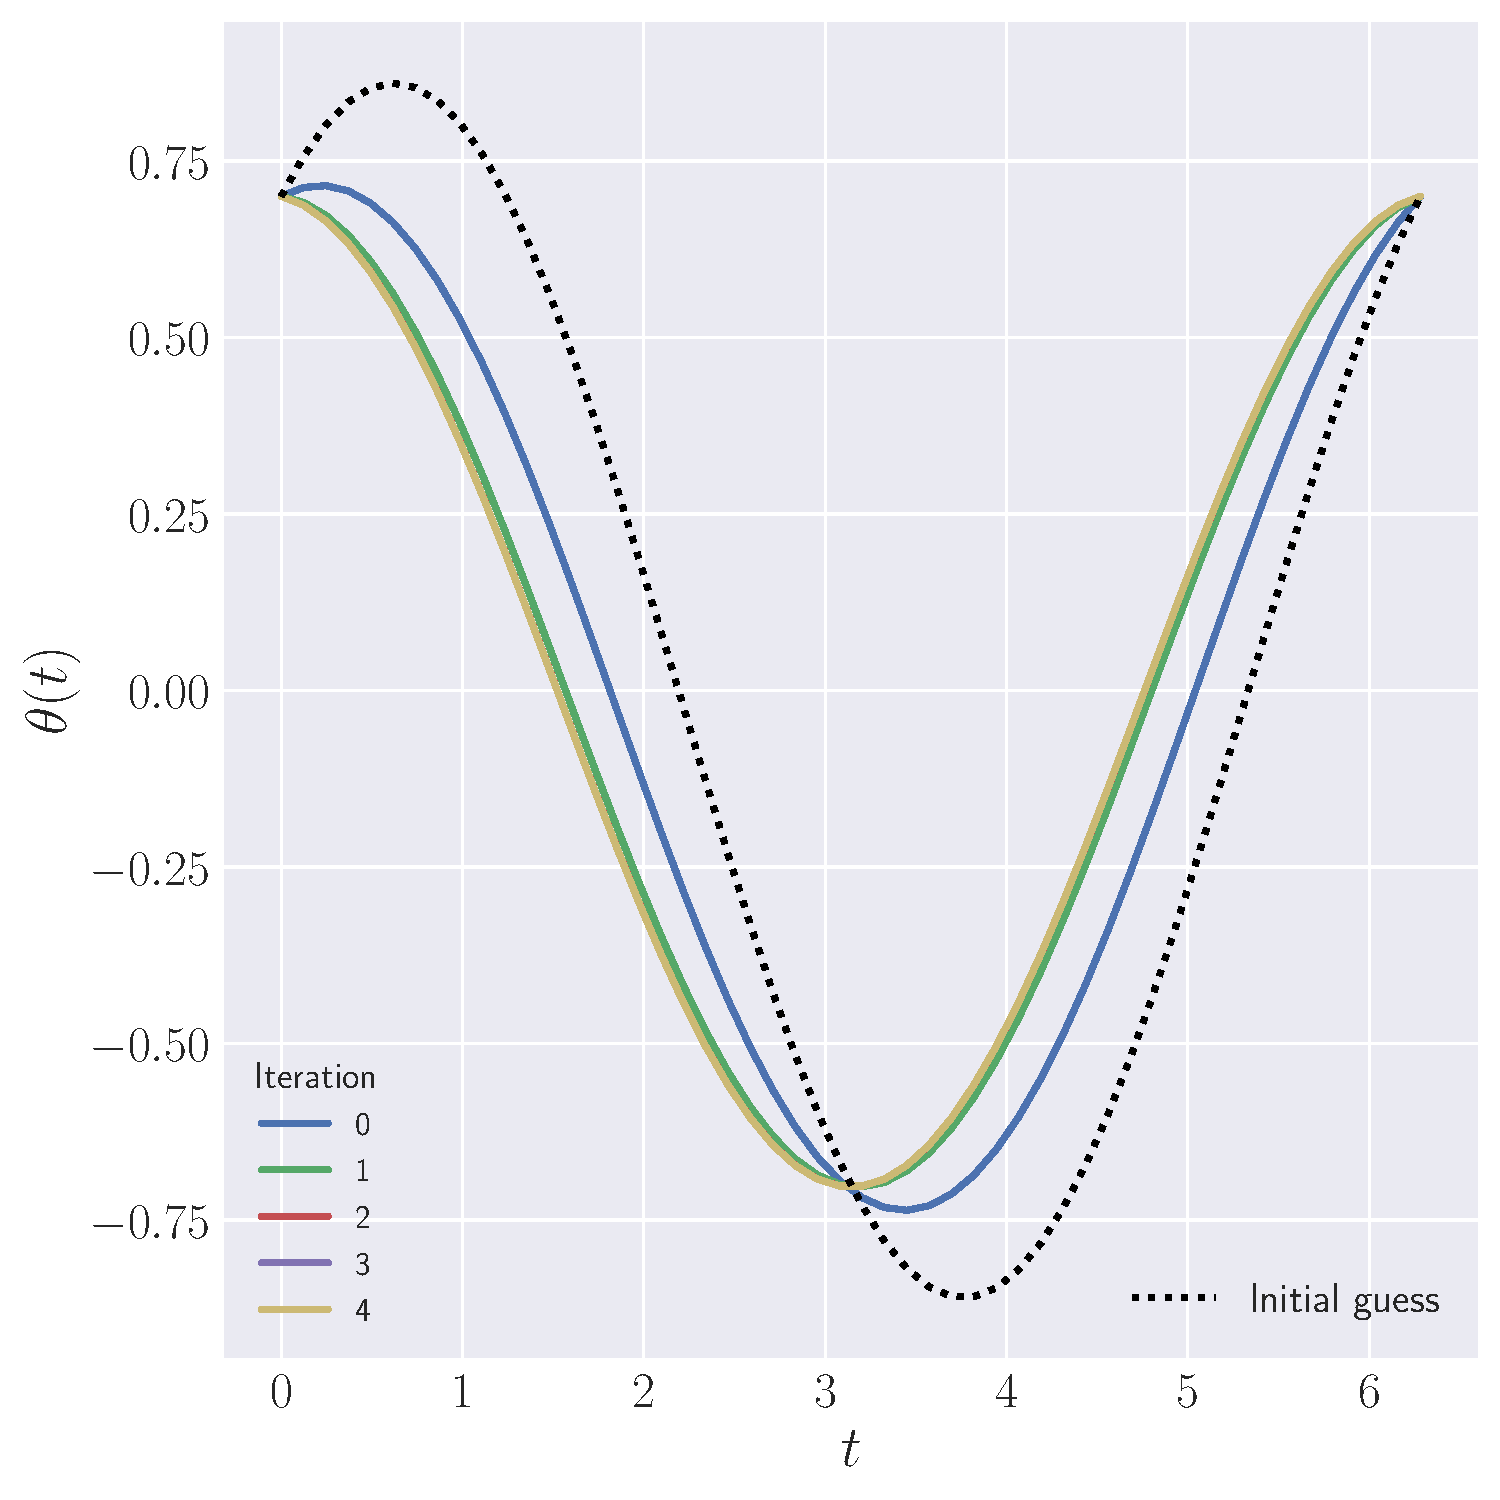
\includegraphics[clip,scale=0.3]{q1a_iteration_figure_2pt4.pdf}}
	\subfloat{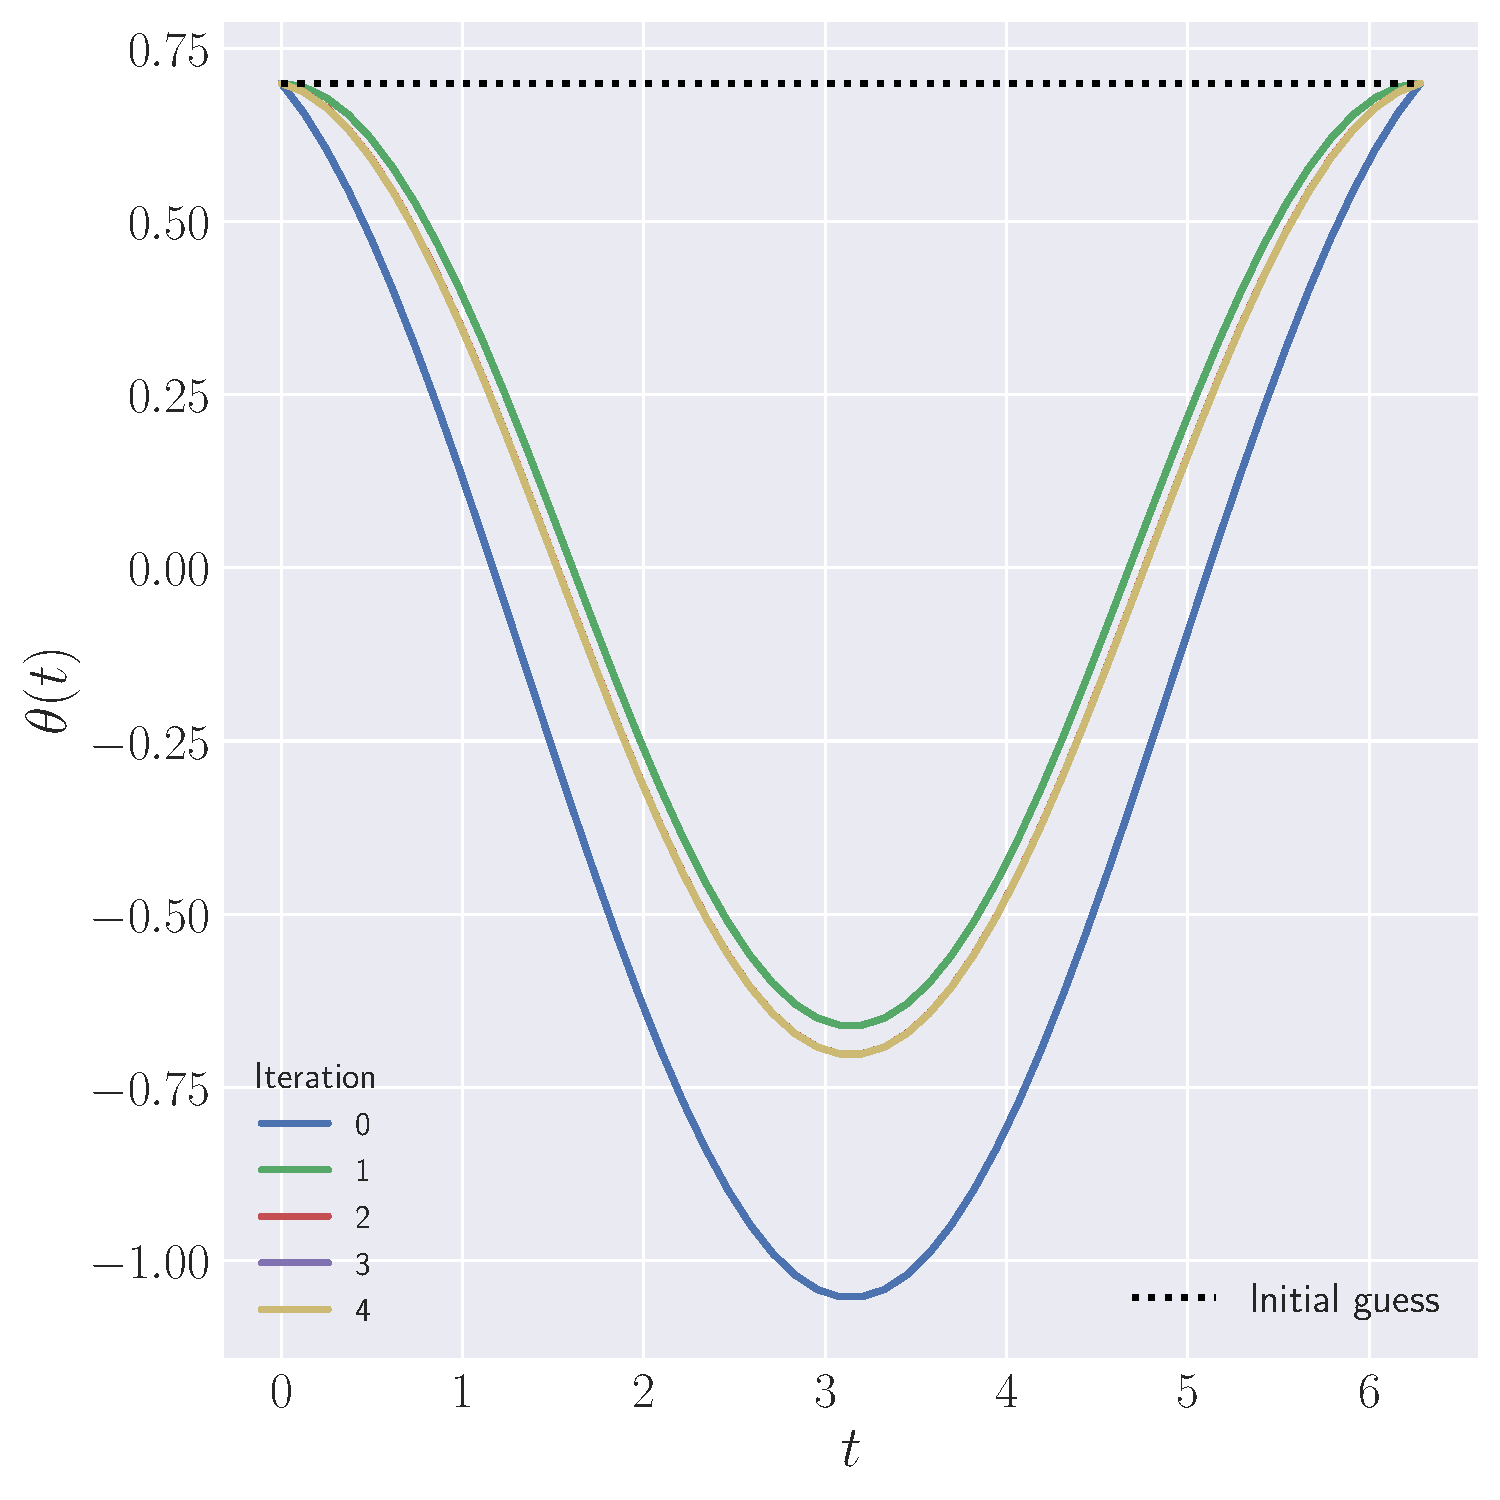
\includegraphics[clip,scale=0.3]{q1a_iteration_figure_2pt4_alt.pdf}}
	
	\subfloat{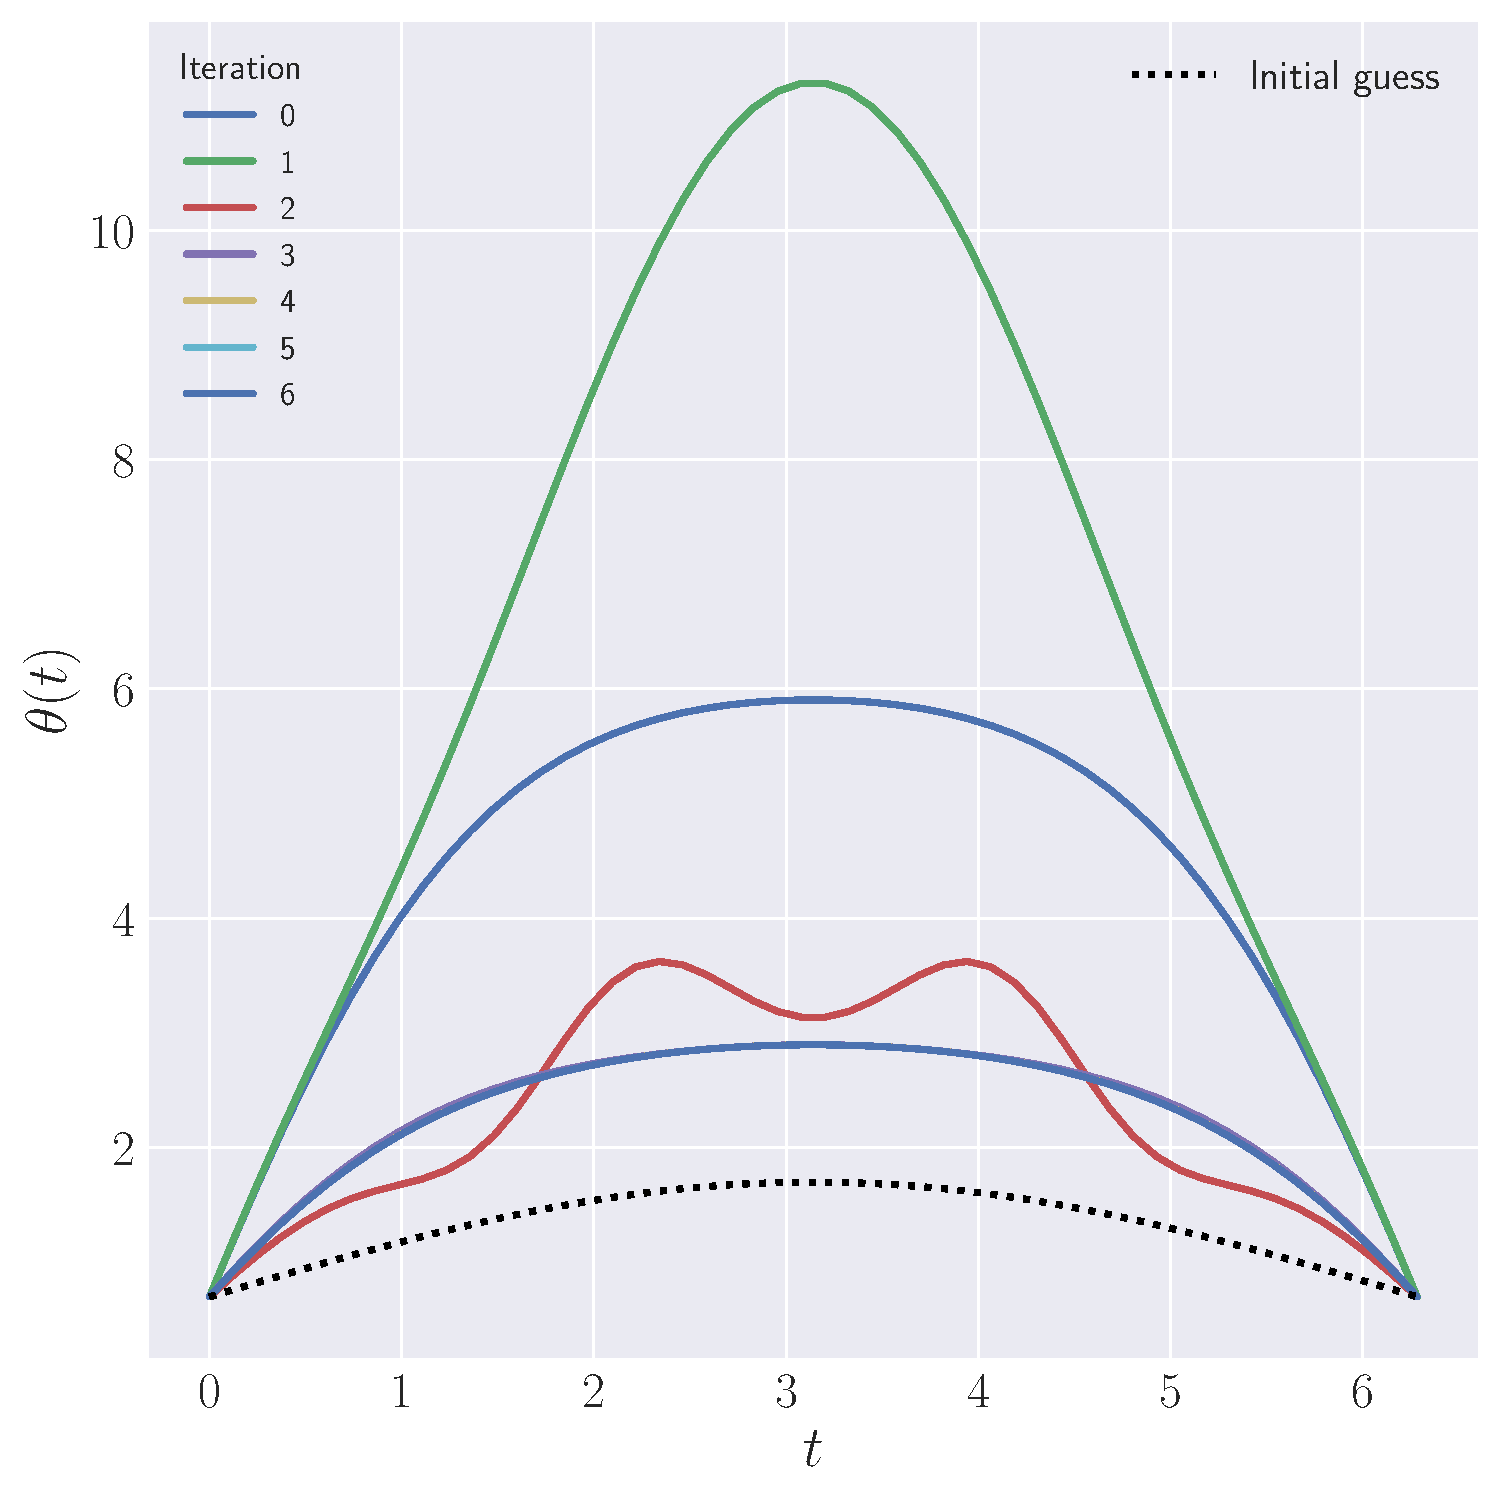
\includegraphics[clip,scale=0.3]{q1a_iteration_figure_2pt5.pdf}}
	\caption{
		Recreation of Fig. 2.4 and Fig. 2.5 from \textbf{[LV]}.
		Angle $\theta$ as a function of time $t$. 
		Initial guess is $\Theta_{i}^{[0]} = 0.7+\sin(t_{i}/2)$.
		Different colors denote the iteration. Iteration counter starts from 0, not including initial guess. Initial guess is denoted by the black dotted line.
	}
	\label{fig:2pt4_2pt5_recreation}
\end{figure}

\FloatBarrier

For an alternate initial solution $\theta^{[0]}=0.7\cos(t_{i})+2\sin(t_{i})$, I find an alternate solution shown in Fig.~\ref{fig:q1_alt_guess_plot}. This oscillation is similar to the one found in the top left-hand subplot of Fig.~\ref{fig:2pt4_2pt5_recreation}; however, this has a larger amplitude.

\begin{figure}[!h]
	\centering
	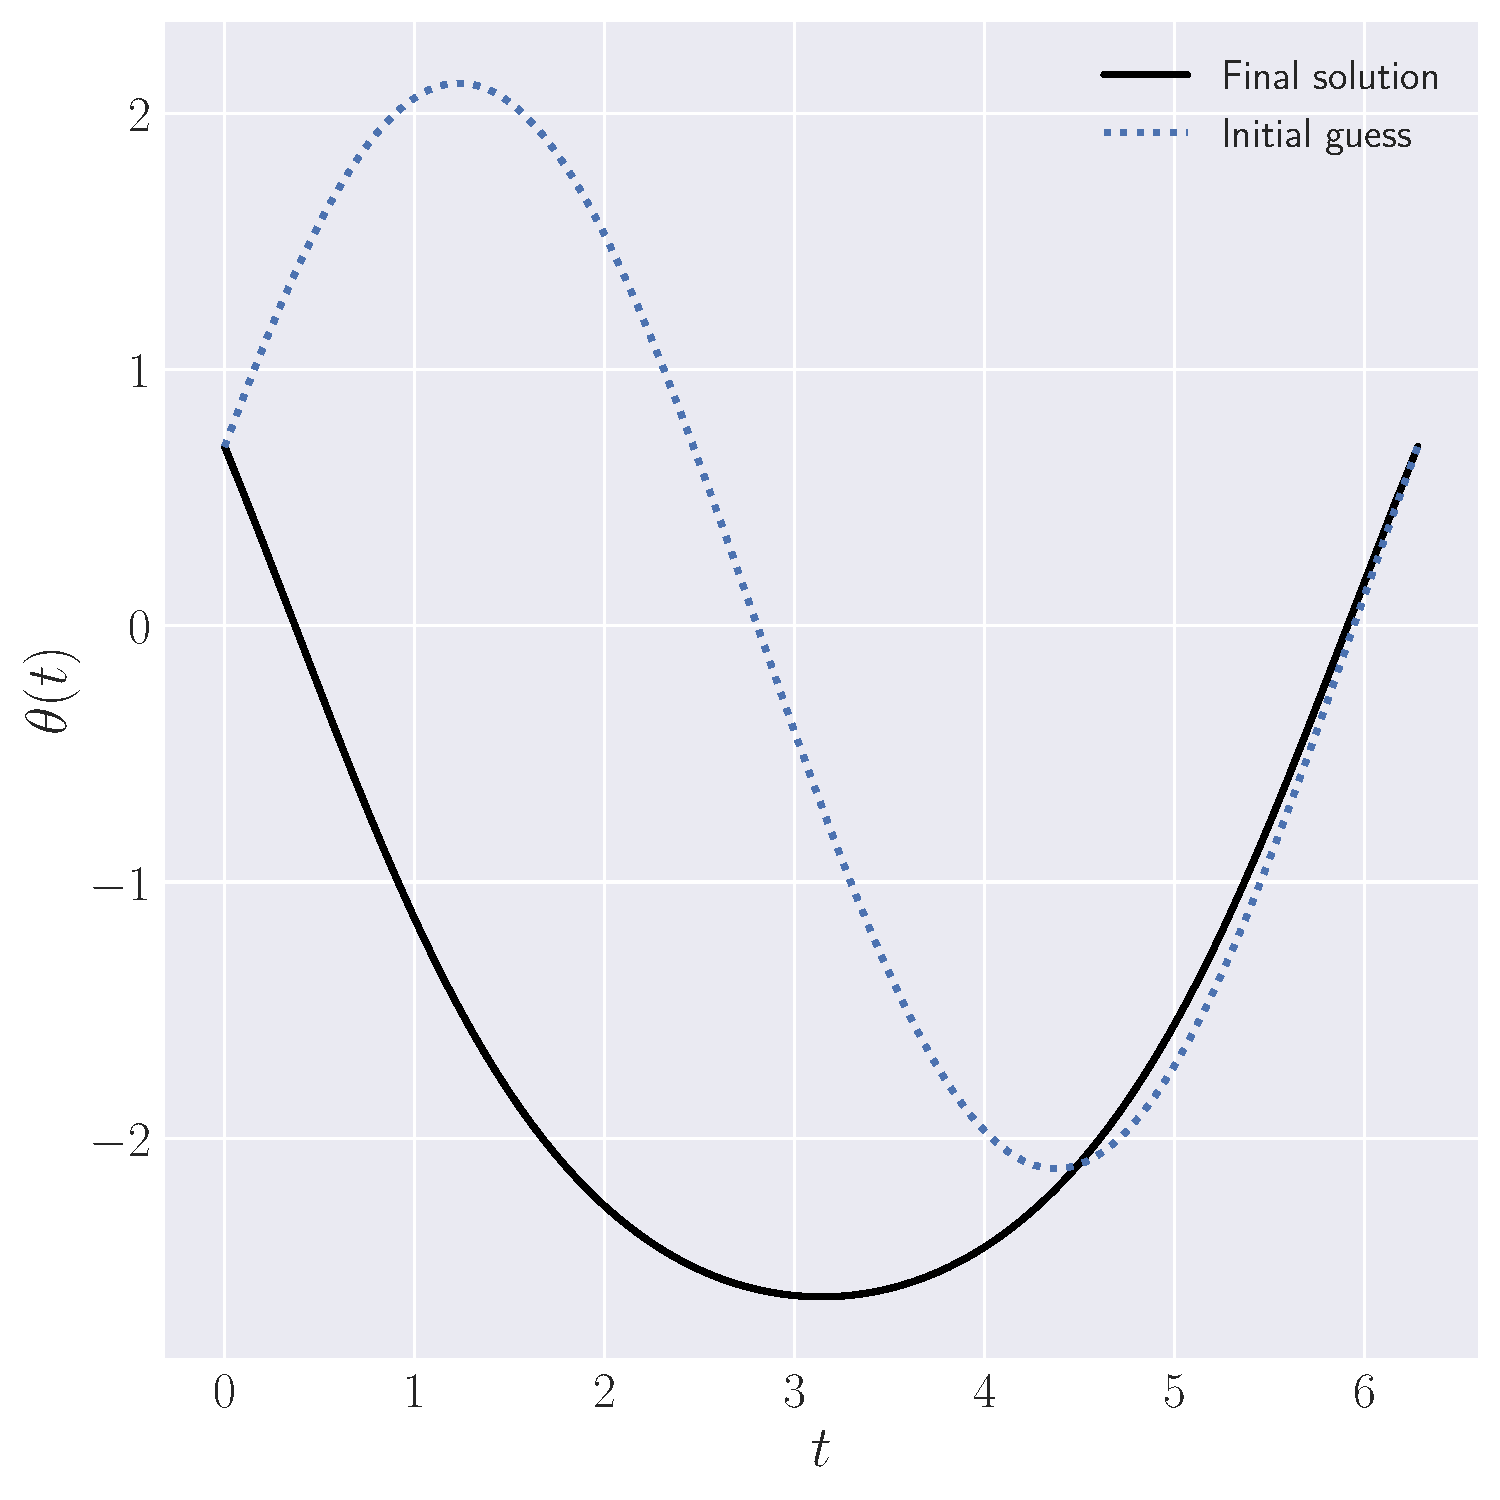
\includegraphics[clip, scale=0.3]{q1a_alt_guess_figure.pdf}
	\caption{Solution of the Newton Iteration with initial guess $\theta^{[0]}=0.7\cos(t_{i})+2\sin(t_{i})$. Dashed blue line denotes the 
	form of the initial guess, while the black solid line denotes the final solution found by the Newton iterator.}
	\label{fig:q1_alt_guess_plot}
\end{figure}

\subsection*{Part B}
For longer time intervals, say $T = 20$, I find the following solution shown in Fig.~\ref{fig:q1b_long} using the initial guess of $\theta^{[0]}=0.9\cos(t_{i})+0.2\sin(t_{i})$.

\begin{figure}
	\centering
	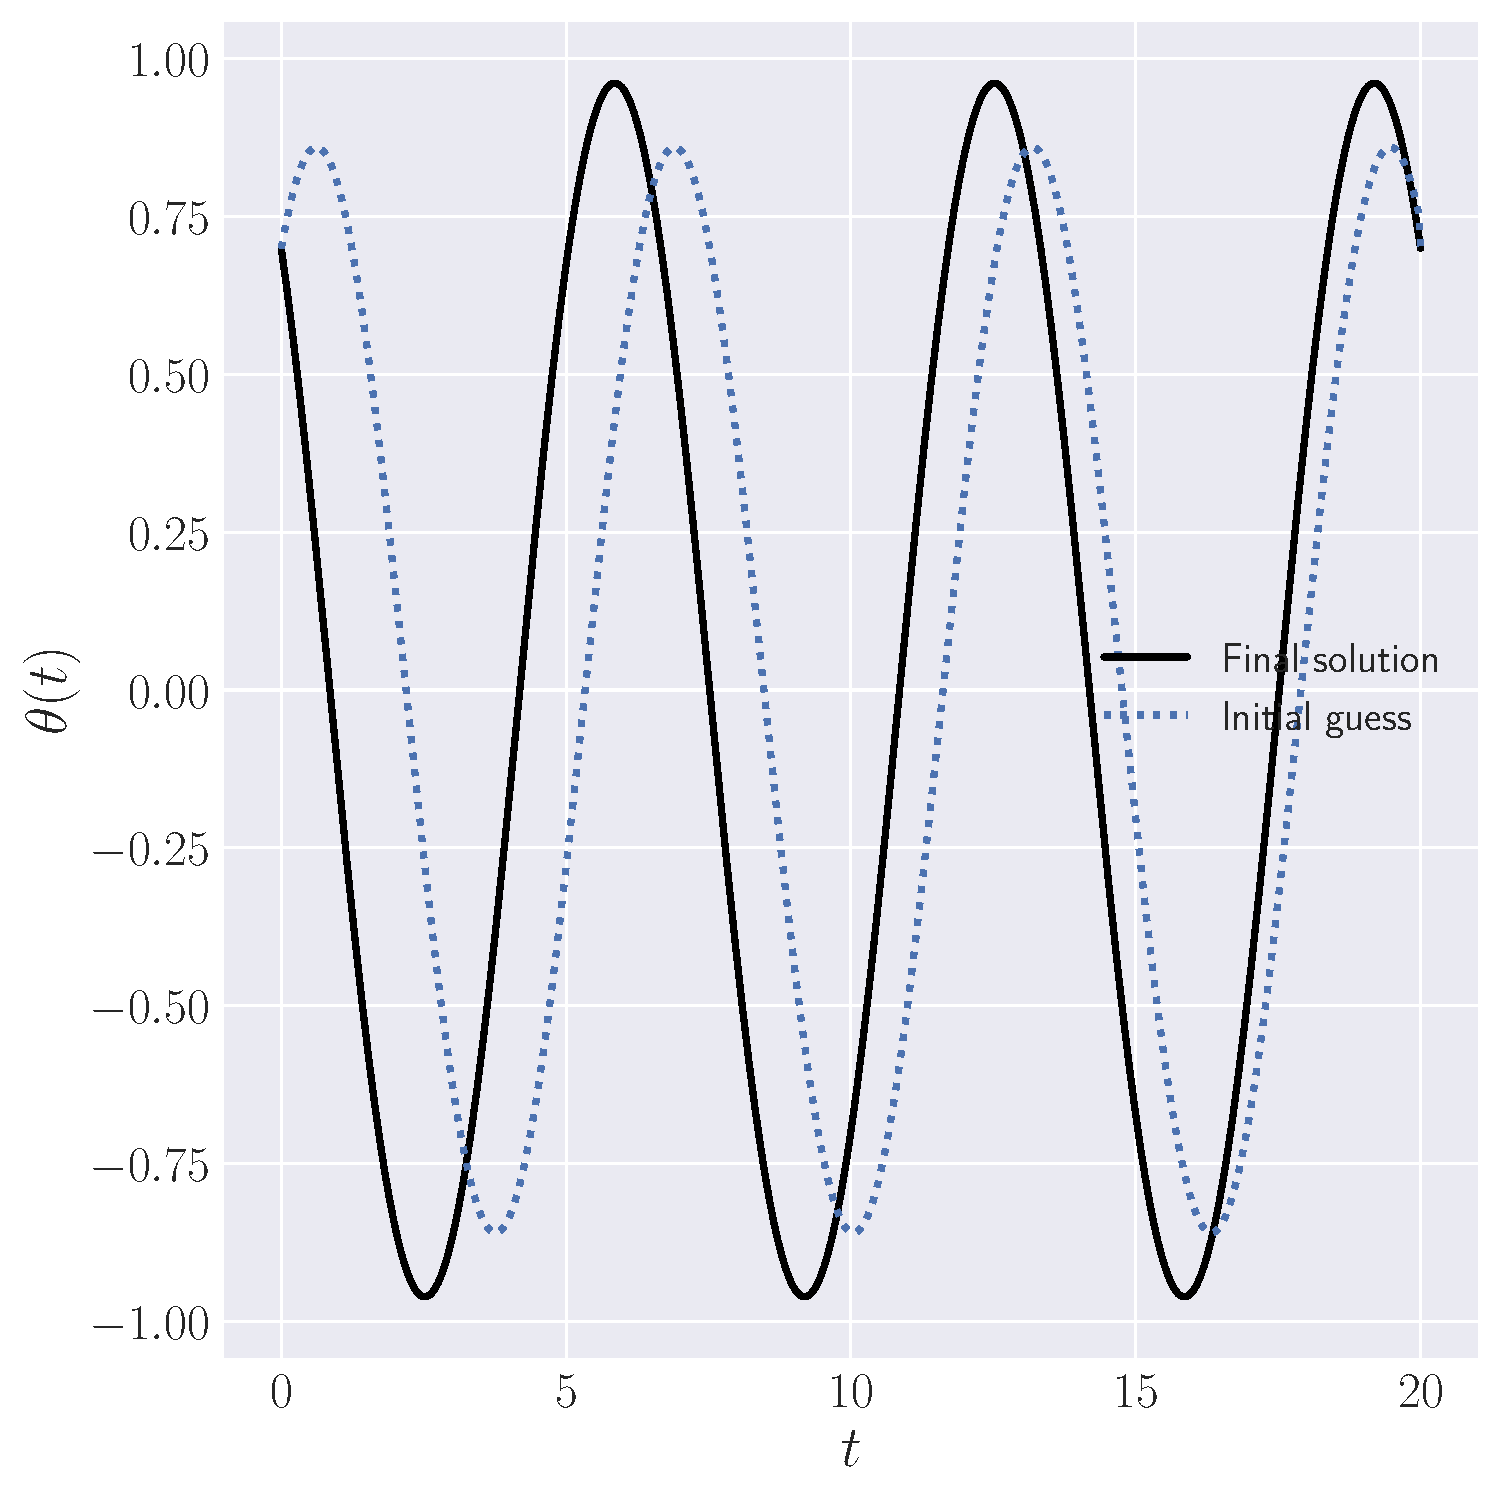
\includegraphics[clip,scale=0.3]{q1b_long_figure.pdf}
    \caption{
        Solution found by the Newton Iteration for $T=20$ using the initial solution $\theta^{[0]}=0.9\cos(t_{i})+0.2\sin(t_{i})$.
        Black solid line denotes the final solution after the convergence criterion was met. The dotted blue line denotes the initial guess
        input into the solver.
    }
    \label{fig:q1b_long}
\end{figure}

In general, as I anticipate the existence of the boundary layer, and from physical intuition I expect that such a solution to be slow moving near $\theta=\pi$, then propose an initial solution 
\begin{align}
	\theta^{[0]} = 
	\begin{cases}
		0.7,&\quad t=0\ \&\ t=T\\
		\pi,&\quad 0 < t < T.
	\end{cases}\label{eq:theta_init}
\end{align}
Doing the Newton iteration with this guess gives a solution found in the left-hand subplot of Fig.~\ref{fig:q1b_scan}. Then scanning across a bunch of different end times $T$, we find (right-hand subplot of Fig.~\ref{fig:q1b_scan}) that the $\max \theta$ asymptotes towards a value of $\theta = \pi$ as we can expect from physical intuition. 

\begin{figure}
    \centering
    \subfloat{\includegraphics[clip,scale=0.3]{q1b_boundary_figure.pdf}}
    \subfloat{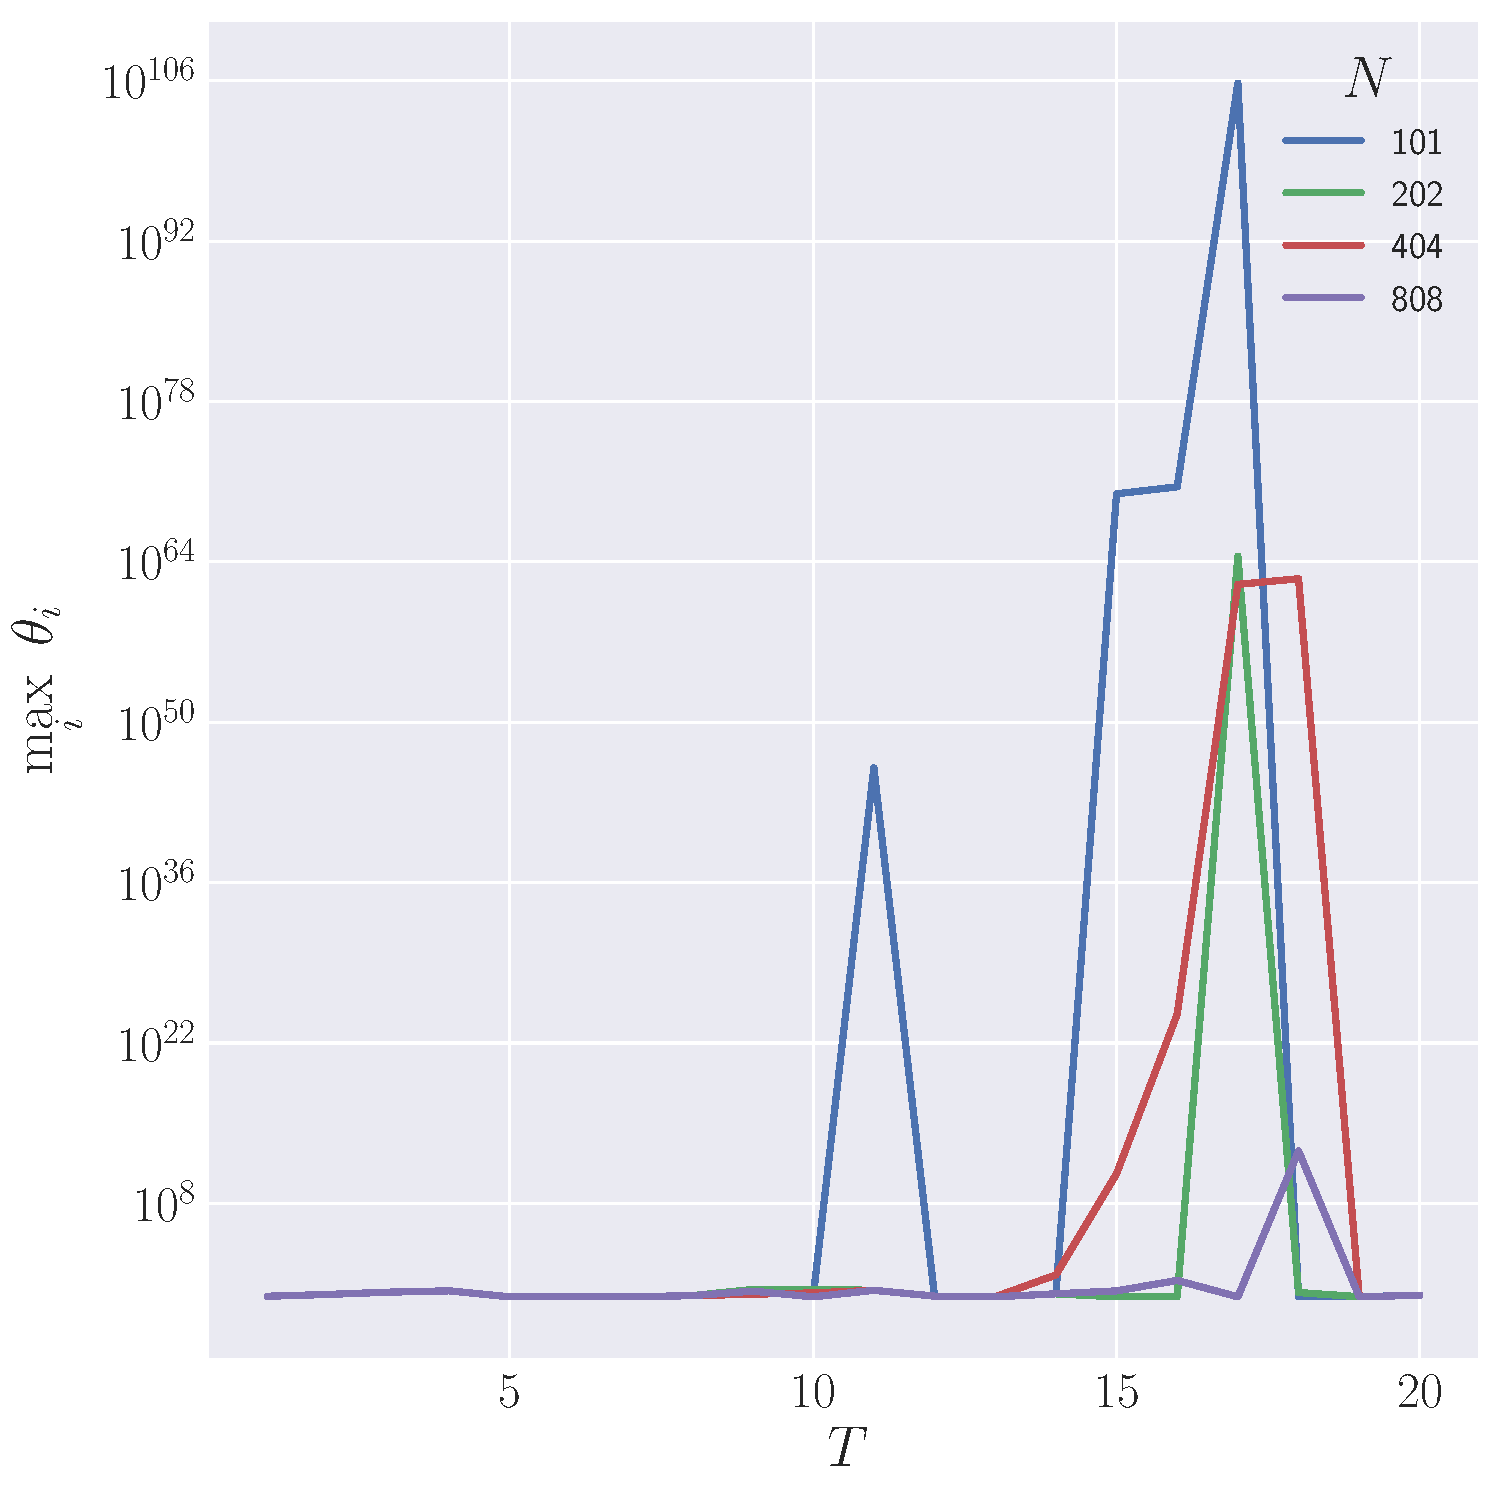
\includegraphics[clip,scale=0.3]{q1b_figure.pdf}}
    \caption{
        [Left Subplot] Solution found by the Newton Iteration for a range of $T$ and for a variety of meshes with differing number of points $m$. [Right Subplot] Solution found by the Newton Iteration for a range of $T$ and for a variety of meshes with differing number of points $m$. Using the initial solution given by~\eqref{eq:theta_init}. Different colors of lines denote different number of mesh points, which are indistinguishable in this case as each converges to the same answer. 
        Blue dashed line denotes the value of $\pi$.
    }
    \label{fig:q1b_scan}
\end{figure}

\section*{Problem 2}

\subsection*{Part A}
I implemented the five-point Laplacian by taking the code that was available on Canvas, translating it into Python, and then modifying the boundary conditions.
This code can be found in the ipython notebook \verb|A2Q2.ipynb|. Figure~\ref{fig:five_pt_soln_recreation} shows the results of this implementation by reproducing all of the example figures in the provided MATLAB code. 

\begin{figure}[!h]
	\centering
	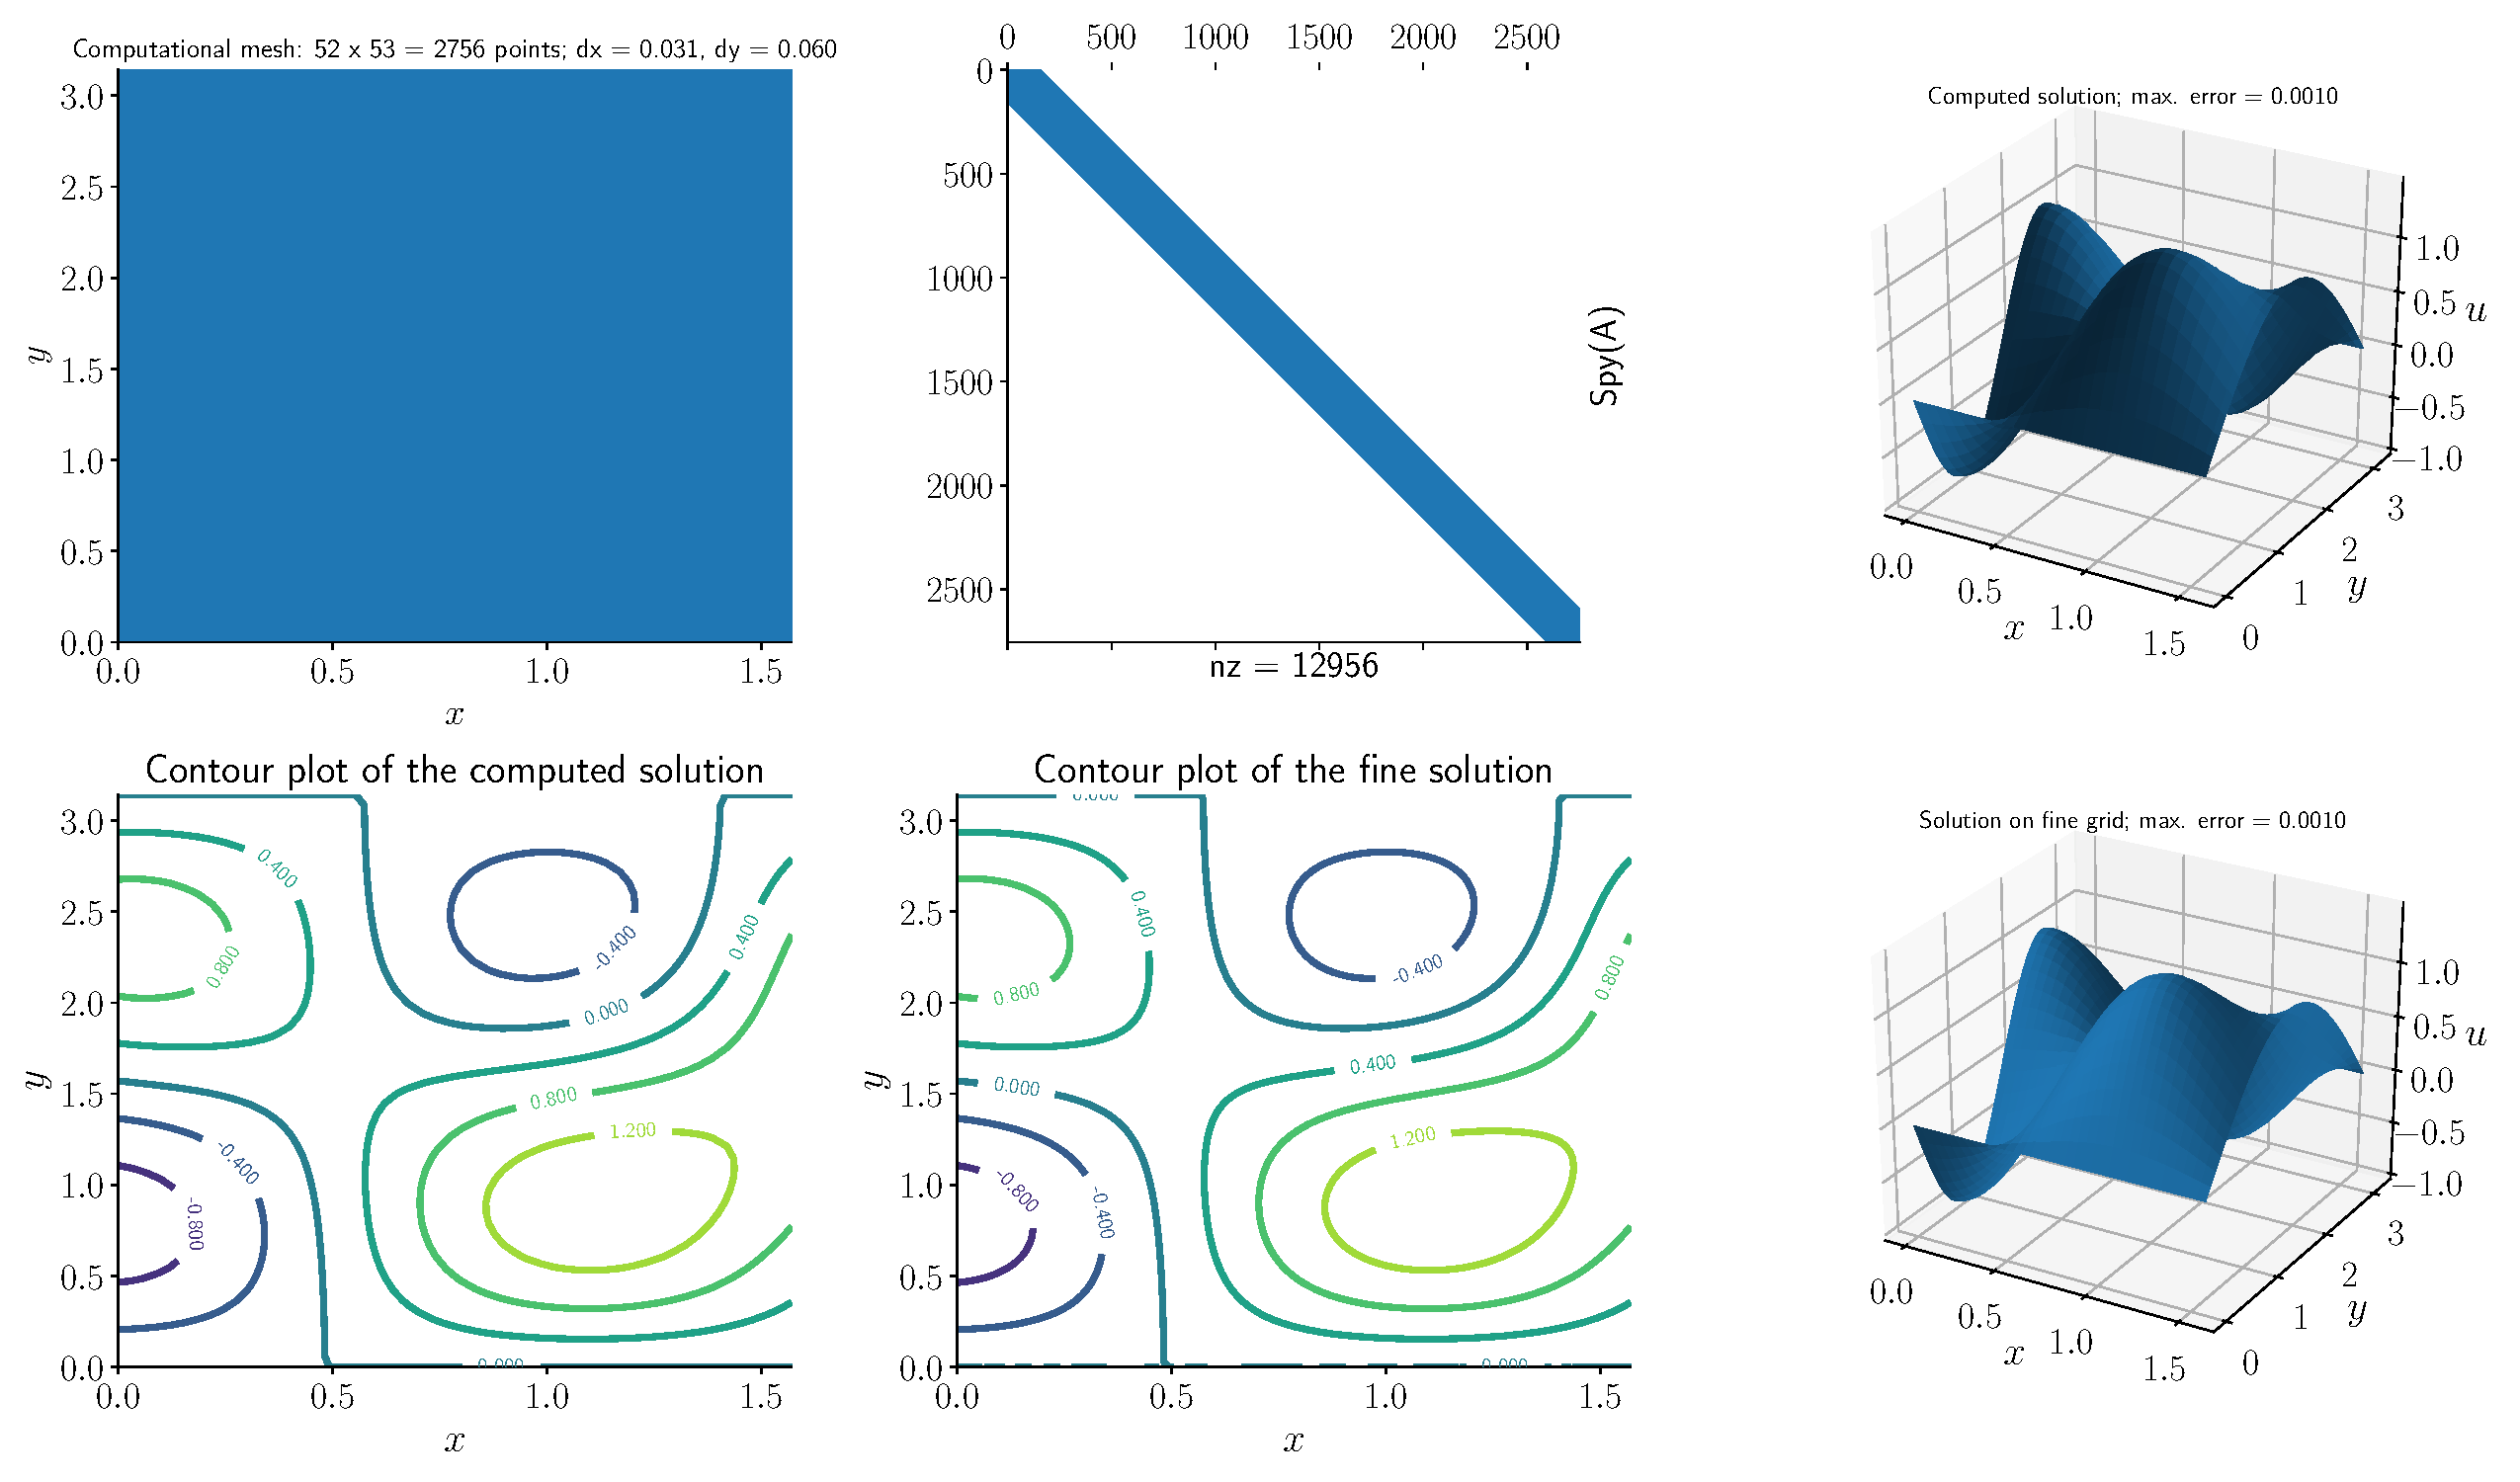
\includegraphics[clip,scale=0.4]{q2a_figure.pdf}
	\caption{Recreation of the example plots for the differential equation $\nabla^{2}u = 13\cos3x\sin2y$, using the five-point Laplacian.}
	\label{fig:five_pt_soln_recreation}
\end{figure}

Performing grid refinement using this implementation of the five-point Laplacian, we observe in Fig.~\ref{fig:five_pt_err_scaling} that this implementation has accuracy of order two. From the grid refinement procedure I estimate that the number of points needed to reach an inf-norm error of $<10^{-5}$ is about 400 points

\begin{figure}[!h]
	\centering
	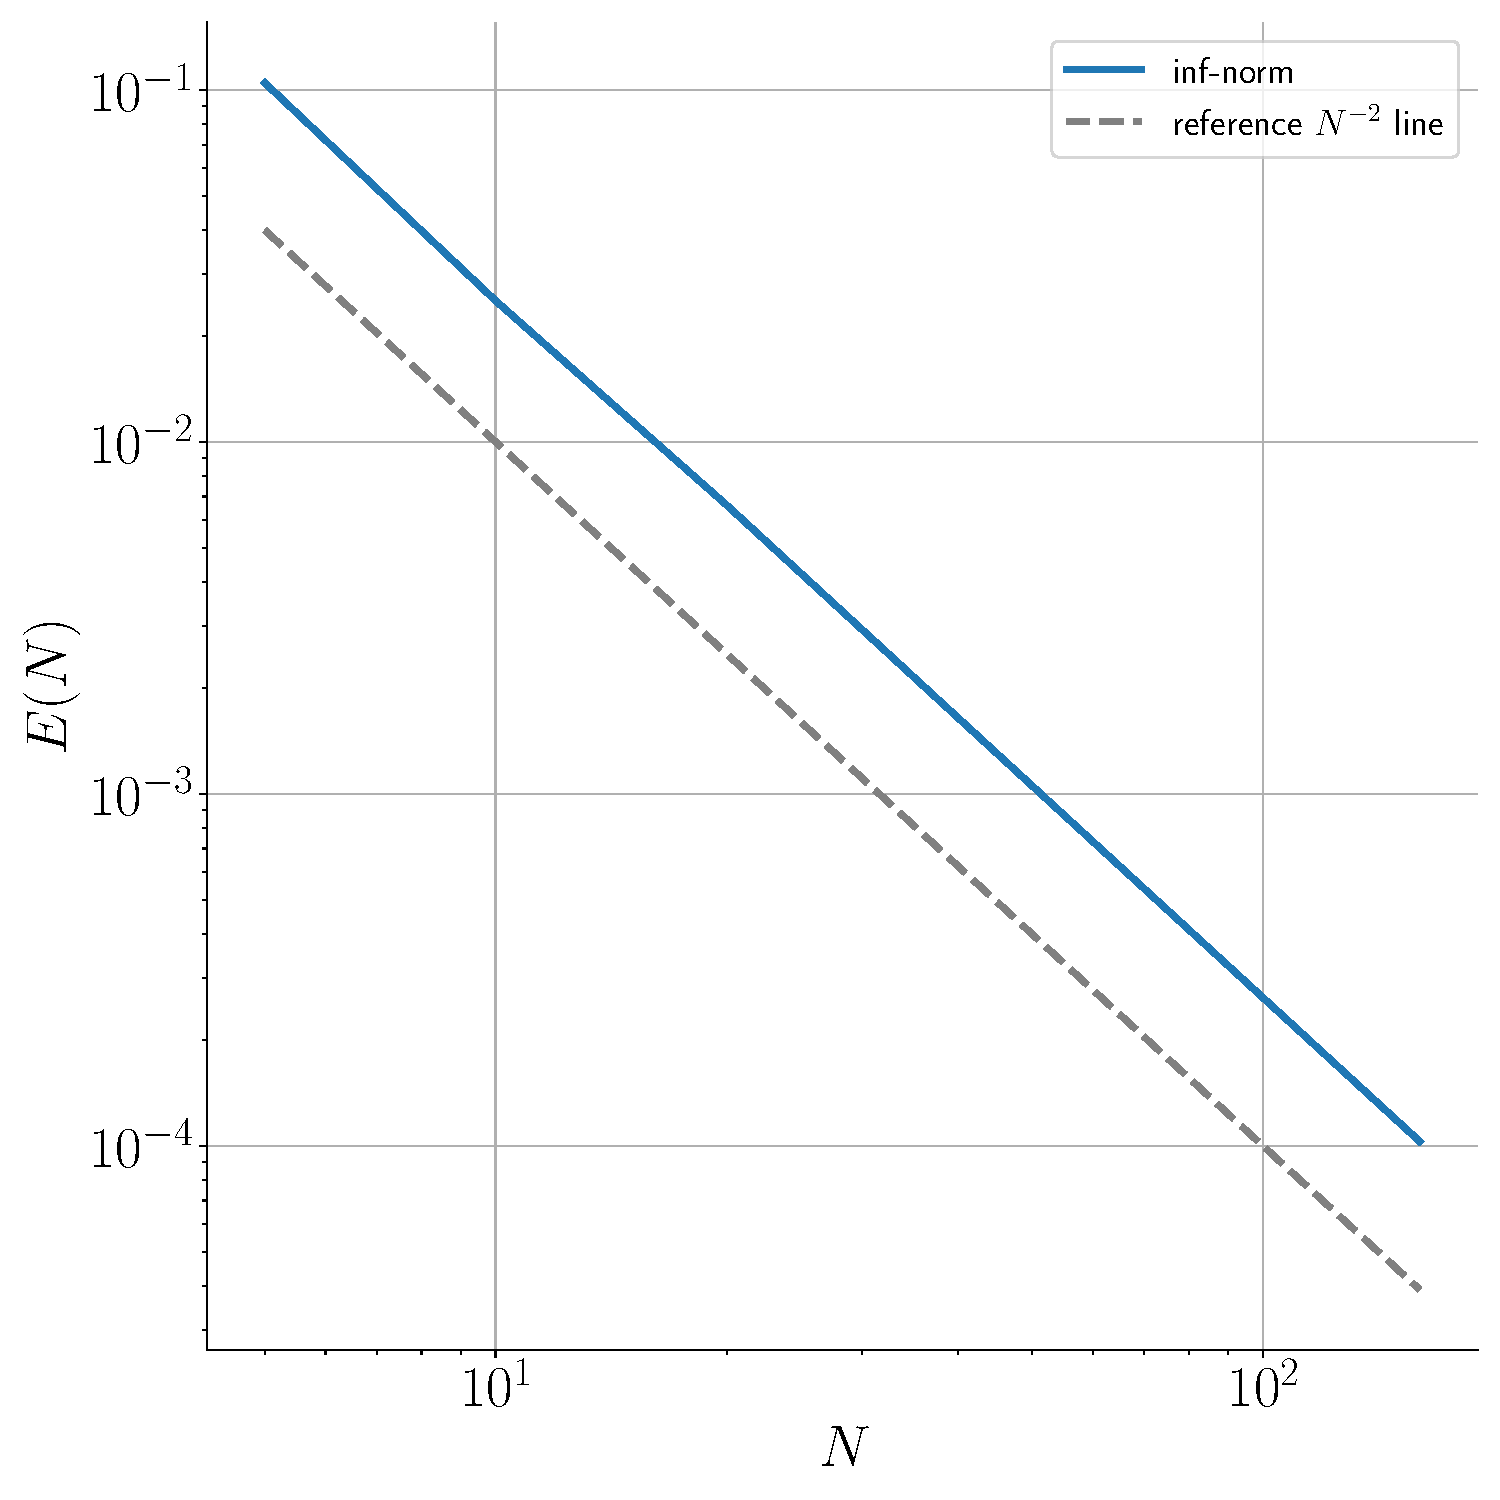
\includegraphics[clip,scale=0.4]{q2a_err_fig.pdf}
	\caption{Error, $E(N)$, as a function of the number of mesh intervals, $N$, for the five-point Laplacian. We observe the desired order of two for this method.}
	\label{fig:five_pt_err_scaling}
\end{figure}

\subsection*{Part B}

The nine-point Laplacian is given by the formula
\begin{align}
	\nabla^{2}_{9}u_{ij} = \dfrac{1}{6h^{2}}\left[
	4(u_{i-1,j}+u_{i+1,j}+u_{i,j-1}+u_{i,j+1})
	+ (u_{i+1,j-1}+u_{i+1,j+1}+u_{i-1,j-1}+u_{i-1,j+1})
	- 20u_{ij}
	\right]\label{eq:npl_equation}
\end{align}

To derive the truncation error we Taylor expand each of the $u_{ij}$. To simplify notation we define the shorthand,
\begin{align}
	u^{(m,n)}(\xbar,\ybar)\equiv \left.\dfrac{\partial^{m+n}}{\partial x^{m}\partial y^{n}}u(x,y)\right|_{x=\xbar,y=\ybar}.
\end{align}
Then, expanding each of the terms in~\eqref{eq:npl_equation}, we have
\begin{subequations}
	\begin{align}
		u_{i-1,j} &= u(\xbar,\ybar)-h u^{(1,0)}(\xbar,\ybar)+\frac{1}{2} h^2 u^{(2,0)}(\xbar,\ybar)-\frac{1}{6} h^3 u^{(3,0)}(\xbar,\ybar)+\frac{1}{24}	h^4 u^{(4,0)}(\xbar,\ybar)\nonumber\\
		&\hspace{9cm}-\frac{1}{120} h^5u^{(5,0)}(\xbar,\ybar)+\bO\left(h^6\right)\\	
		%%%%%%%%%%%%%%%%%%%%%%%%%%%%%%%%%%%%%%%%%%%%%%%%%%%%%%%%%%%%%%%%%%%%%%%
		u_{i+1,j} &= u(\xbar,\ybar)+h u^{(1,0)}(\xbar,\ybar)+\frac{1}{2} h^2 u^{(2,0)}(\xbar,\ybar)+\frac{1}{6} h^3 u^{(3,0)}(\xbar,\ybar)+\frac{1}{24}
		h^4 u^{(4,0)}(\xbar,\ybar)\nonumber\\
		&\hspace{9cm}+\frac{1}{120} h^5u^{(5,0)}(\xbar,\ybar)+\bO\left(h^6\right)\\
		%%%%%%%%%%%%%%%%%%%%%%%%%%%%%%%%%%%%%%%%%%%%%%%%%%%%%%%%%%%%%%%%%%%%%%%
		u_{i,j-1} &= u(\xbar,\ybar)-h u^{(0,1)}(\xbar,\ybar)+\frac{1}{2} h^2 u^{(0,2)}(\xbar,\ybar)-\frac{1}{6} h^3 u^{(0,3)}(\xbar,\ybar)+\frac{1}{24}
		h^4 u^{(0,4)}(\xbar,\ybar)\nonumber\\
		&\hspace{9cm}-\frac{1}{120} h^5u^{(0,5)}(\xbar,\ybar)+\bO\left(h^6\right)\\
		%%%%%%%%%%%%%%%%%%%%%%%%%%%%%%%%%%%%%%%%%%%%%%%%%%%%%%%%%%%%%%%%%%%%%%%
		u_{i,j+1} &= u(\xbar,\ybar)+h u^{(0,1)}(\xbar,\ybar)+\frac{1}{2} h^2 u^{(0,2)}(\xbar,\ybar)+\frac{1}{6} h^3 u^{(0,3)}(\xbar,\ybar)+\frac{1}{24}
		h^4 u^{(0,4)}(\xbar,\ybar)\nonumber\\
		&\hspace{9cm}+\frac{1}{120} h^5u^{(0,5)}(\xbar,\ybar)+\bO\left(h^6\right)
	\end{align}
\end{subequations}
Adding these equations to compute the first group of terms inside the bracket of~\eqref{eq:npl_equation} we have that
\begin{align}
	4(u_{i-1,j}+u_{i+1,j}+u_{i,j-1}+u_{i,j+1}) &= 16 u(\xbar,\ybar)
	+4 h^2 \left(u^{(0,2)}(\xbar,\ybar)
	+u^{(2,0)}(\xbar,\ybar)\right)\nonumber\\
	&\hspace{3cm}+\frac{1}{3} h^4\left(u^{(0,4)}(\xbar,\ybar)
	+u^{(4,0)}(\xbar,\ybar)\right)
	+\bO\left(h^6\right)\label{eq:npl_grp1}
\end{align}
Computing the expansions of the remaining terms we have
\begin{subequations}
	\begin{align}
		u_{i-1,j-1} &= u(\xbar,\ybar)+
		h\left(-u^{(0,1)}(\xbar,\ybar)-u^{(1,0)}(\xbar,\ybar)\right)
		+\frac{1}{2}h^2 \left(u^{(0,2)}(\xbar,\ybar)+2		u^{(1,1)}(\xbar,\ybar)+u^{(2,0)}(\xbar,\ybar)\right)\nonumber\\
		&\hspace{1.5cm}-\frac{1}{6} h^3 \left(u^{(0,3)}(\xbar,\ybar) +3\left(u^{(1,2)}(\xbar,\ybar)+u^{(2,1)}(\xbar,\ybar)\right)+u^{(3,0)}(\xbar,\ybar)\right)\nonumber\\
		&\hspace{1.5cm}+\frac{1}{24} h^4
		\left(u^{(0,4)}(\xbar,\ybar)+4 u^{(1,3)}(\xbar,\ybar)+6 u^{(2,2)}(\xbar,\ybar)+4
		u^{(3,1)}(\xbar,\ybar)+u^{(4,0)}(\xbar,\ybar)\right)\nonumber\\
		&-\frac{1}{120} h^5 \left(u^{(0,5)}(\xbar,\ybar)+5
		\left(u^{(1,4)}(\xbar,\ybar)+2
		\left(u^{(2,3)}(\xbar,\ybar)+u^{(3,2)}(\xbar,\ybar)\right)+u^{
			(4,1)}(\xbar,\ybar)\right)+u^{(5,0)}(\xbar,\ybar)\right)\nonumber\\
		&+\bO\left(h^6\right)\\
		%%%%%%%%%%%%%%%%%%%%%%%%%%%%%%%%%%%%%%%%%%%%%%%%%%%%%%%%%%%%%%%%%%%%%%%
		u_{i-1,j+1} &= u(\xbar,\ybar)
		+h\left(u^{(0,1)}(\xbar,\ybar)-u^{(1,0)}(\xbar,\ybar)\right)
		+\frac{1}{2} h^2 \left(u^{(0,2)}(\xbar,\ybar)-2		u^{(1,1)}(\xbar,\ybar)+u^{(2,0)}(\xbar,\ybar)\right)\nonumber\\
		&\hspace{1.5cm}+\frac{1}{6} h^3 \left(u^{(0,3)}(\xbar,\ybar)-3 u^{(1,2)}(\xbar,\ybar)+3u^{(2,1)}(\xbar,\ybar)-u^{(3,0)}(\xbar,\ybar)\right)\nonumber\\
		&\hspace{1.5cm}+\frac{1}{24} h^4 \left(u^{(0,4)}(\xbar,\ybar)-4 u^{(1,3)}(\xbar,\ybar)+6u^{(2,2)}(\xbar,\ybar)-4 u^{(3,1)}(\xbar,\ybar)+u^{(4,0)}(\xbar,\ybar)\right)\nonumber\\
		&+\frac{1}{
			120} h^5 \left(u^{(0,5)}(\xbar,\ybar)-5
		u^{(1,4)}(\xbar,\ybar)+5 \left(2 u^{(2,3)}(\xbar,\ybar)-2
		u^{(3,2)}(\xbar,\ybar)+u^{(4,1)}(\xbar,\ybar)\right)-u^{(5,0)}
		(\xbar,\ybar)\right)\nonumber\\
		&+\bO\left(h^6\right)\\
		%%%%%%%%%%%%%%%%%%%%%%%%%%%%%%%%%%%%%%%%%%%%%%%%%%%%%%%%%%%%%%%%%%%%%%%
		u_{i+1,j-1} &= u(\xbar,\ybar)
		+h\left(u^{(1,0)}(\xbar,\ybar)-u^{(0,1)}(\xbar,\ybar)\right)
		+\frac{1}{2} h^2 \left(u^{(0,2)}(\xbar,\ybar)-2		u^{(1,1)}(\xbar,\ybar)+u^{(2,0)}(\xbar,\ybar)\right)\nonumber\\
		&\hspace{1.5cm}-\frac{1}{6} h^3 \left(u^{(0,3)}(\xbar,\ybar)-3 u^{(1,2)}(\xbar,\ybar)+3u^{(2,1)}(\xbar,\ybar)-u^{(3,0)}(\xbar,\ybar)\right)\nonumber\\
		&\hspace{1.5cm}+\frac{1}{24} h^4 \left(u^{(0,4)}(\xbar,\ybar)-4 u^{(1,3)}(\xbar,\ybar)+6u^{(2,2)}(\xbar,\ybar)-4 u^{(3,1)}(\xbar,\ybar)+u^{(4,0)}(\xbar,\ybar)\right)\nonumber\\
		&-\frac{1}{120} h^5 \left(u^{(0,5)}(\xbar,\ybar)-5
		u^{(1,4)}(\xbar,\ybar)+5 \left(2 u^{(2,3)}(\xbar,\ybar)-2
		u^{(3,2)}(\xbar,\ybar)+u^{(4,1)}(\xbar,\ybar)\right)-u^{(5,0)}(\xbar,\ybar)\right)\nonumber\\
		&+\bO\left(h^6\right)\\
		%%%%%%%%%%%%%%%%%%%%%%%%%%%%%%%%%%%%%%%%%%%%%%%%%%%%%%%%%%%%%%%%%%%%%%%
		u_{i+1,j+1} &= u(\xbar,\ybar)
		+h\left(u^{(0,1)}(\xbar,\ybar)+u^{(1,0)}(\xbar,\ybar)\right)
		+\frac{1}{2} h^2 \left(u^{(0,2)}(\xbar,\ybar)+2
		u^{(1,1)}(\xbar,\ybar)+u^{(2,0)}(\xbar,\ybar)\right)\nonumber\\
		&\hspace{1.5cm}+\frac{1}{6} h^3 \left(u^{(0,3)}(\xbar,\ybar)+3		\left(u^{(1,2)}(\xbar,\ybar)+u^{(2,1)}(\xbar,\ybar)\right)+u^{(3,0)}(\xbar,\ybar)\right)\nonumber\\
		&\hspace{1.5cm}+\frac{1}{24} h^4 \left(u^{(0,4)}(\xbar,\ybar)+4 u^{(1,3)}(\xbar,\ybar)+6 u^{(2,2)}(\xbar,\ybar)+4
		u^{(3,1)}(\xbar,\ybar)+u^{(4,0)}(\xbar,\ybar)\right)\nonumber\\
		&+\frac{1}{120} h^5 \left(u^{(0,5)}(\xbar,\ybar)+5
		\left(u^{(1,4)}(\xbar,\ybar)+2
		\left(u^{(2,3)}(\xbar,\ybar)+u^{(3,2)}(\xbar,\ybar)\right)+u^{(4,1)}(\xbar,\ybar)\right)+u^{(5,0)}(\xbar
		,\ybar)\right)\nonumber\\
		&+\bO\left(h^6\right).
	\end{align}
\end{subequations}
Combining these terms to compute the remaining group of terms gives 
\begin{align}
	u_{i+1,j-1}+u_{i+1,j+1}+u_{i-1,j-1}+u_{i-1,j+1} &= 4 u(\xbar,\ybar)
	+2h^2\left(u^{(0,2)}(\xbar,\ybar)+u^{(2,0)}(\xbar,\ybar)\right)\nonumber\\
	&\hspace{1.5cm}+\frac{1}{6} h^4 \left(u^{(0,4)}(\xbar,\ybar)+6	u^{(2,2)}(\xbar,\ybar)+u^{(4,0)}(\xbar,\ybar)\right)
	+\bO\left(h^6\right).\label{eq:npl_grp2}
\end{align}
Substituting~\eqref{eq:npl_grp1} and~\eqref{eq:npl_grp2} into~\eqref{eq:npl_equation} and simplifying yields
\begin{subequations}
	\begin{align}
		\nabla^{2}_{9}u(\xbar,\ybar) &= \left(u^{(0,2)}(\xbar,\ybar)+u^{(2,0)}(\xbar,\ybar)\right)+\frac{1}{12} h^2 \left(u^{(0,4)}(\xbar,\ybar)+2
		u^{(2,2)}(\xbar,\ybar)+u^{(4,0)}(\xbar,\ybar)\right)+\bO\left(h^4\right)\\
		&= \nabla^{2}u(\xbar,\ybar)+\frac{1}{12}h^2 \nabla^{2}\left(\nabla^{2}u(\xbar,\ybar)\right)+\bO\left(h^4\right)\\
		&= \nabla^{2}u(\xbar,\ybar)+\frac{1}{12}h^2 \nabla^{4}u(\xbar,\ybar)+\bO\left(h^4\right)
	\end{align}
\end{subequations}
Computing the truncation error then gives
\begin{align}
	\nabla^{2}_{9}u(\xbar,\ybar) - \nabla^{2}u(\xbar,\ybar) &= \frac{1}{12} h^2 \nabla^{4}u(\xbar,\ybar)+\bO\left(h^4\right).
\end{align}

The nine-point Laplacian is only a valid approximation if the mesh width in both dimensions is equivalent. As such here we set the number of point $m$ to specify the number of internal mesh points in the x-direction and from this we compute the necessary $n$ number of internal mesh points in the y-direction such that the grid spacing in both dimensions are equivalent:
\begin{subequations}
	\begin{align}
		\Delta y &= \Delta x\\
		\dfrac{L_{y}}{n+1} &= \dfrac{L_{x}}{m+1}\\
		\implies n &= \dfrac{L_{y}}{L_{x}}\left[m+1\right]-1.
	\end{align}
\end{subequations}

Implementing this in in the ipython notebook \verb|A2Q2.ipynb|, in the section marked ``Part B''. Figure~\ref{fig:nine_pt_soln_subplots}, shows the recreation of the example plots using the nine-point Laplacian. We see that the implementation successfully reproduces the results acquired from the 5-point Laplacian. 

\begin{figure}[!h]
	\centering
	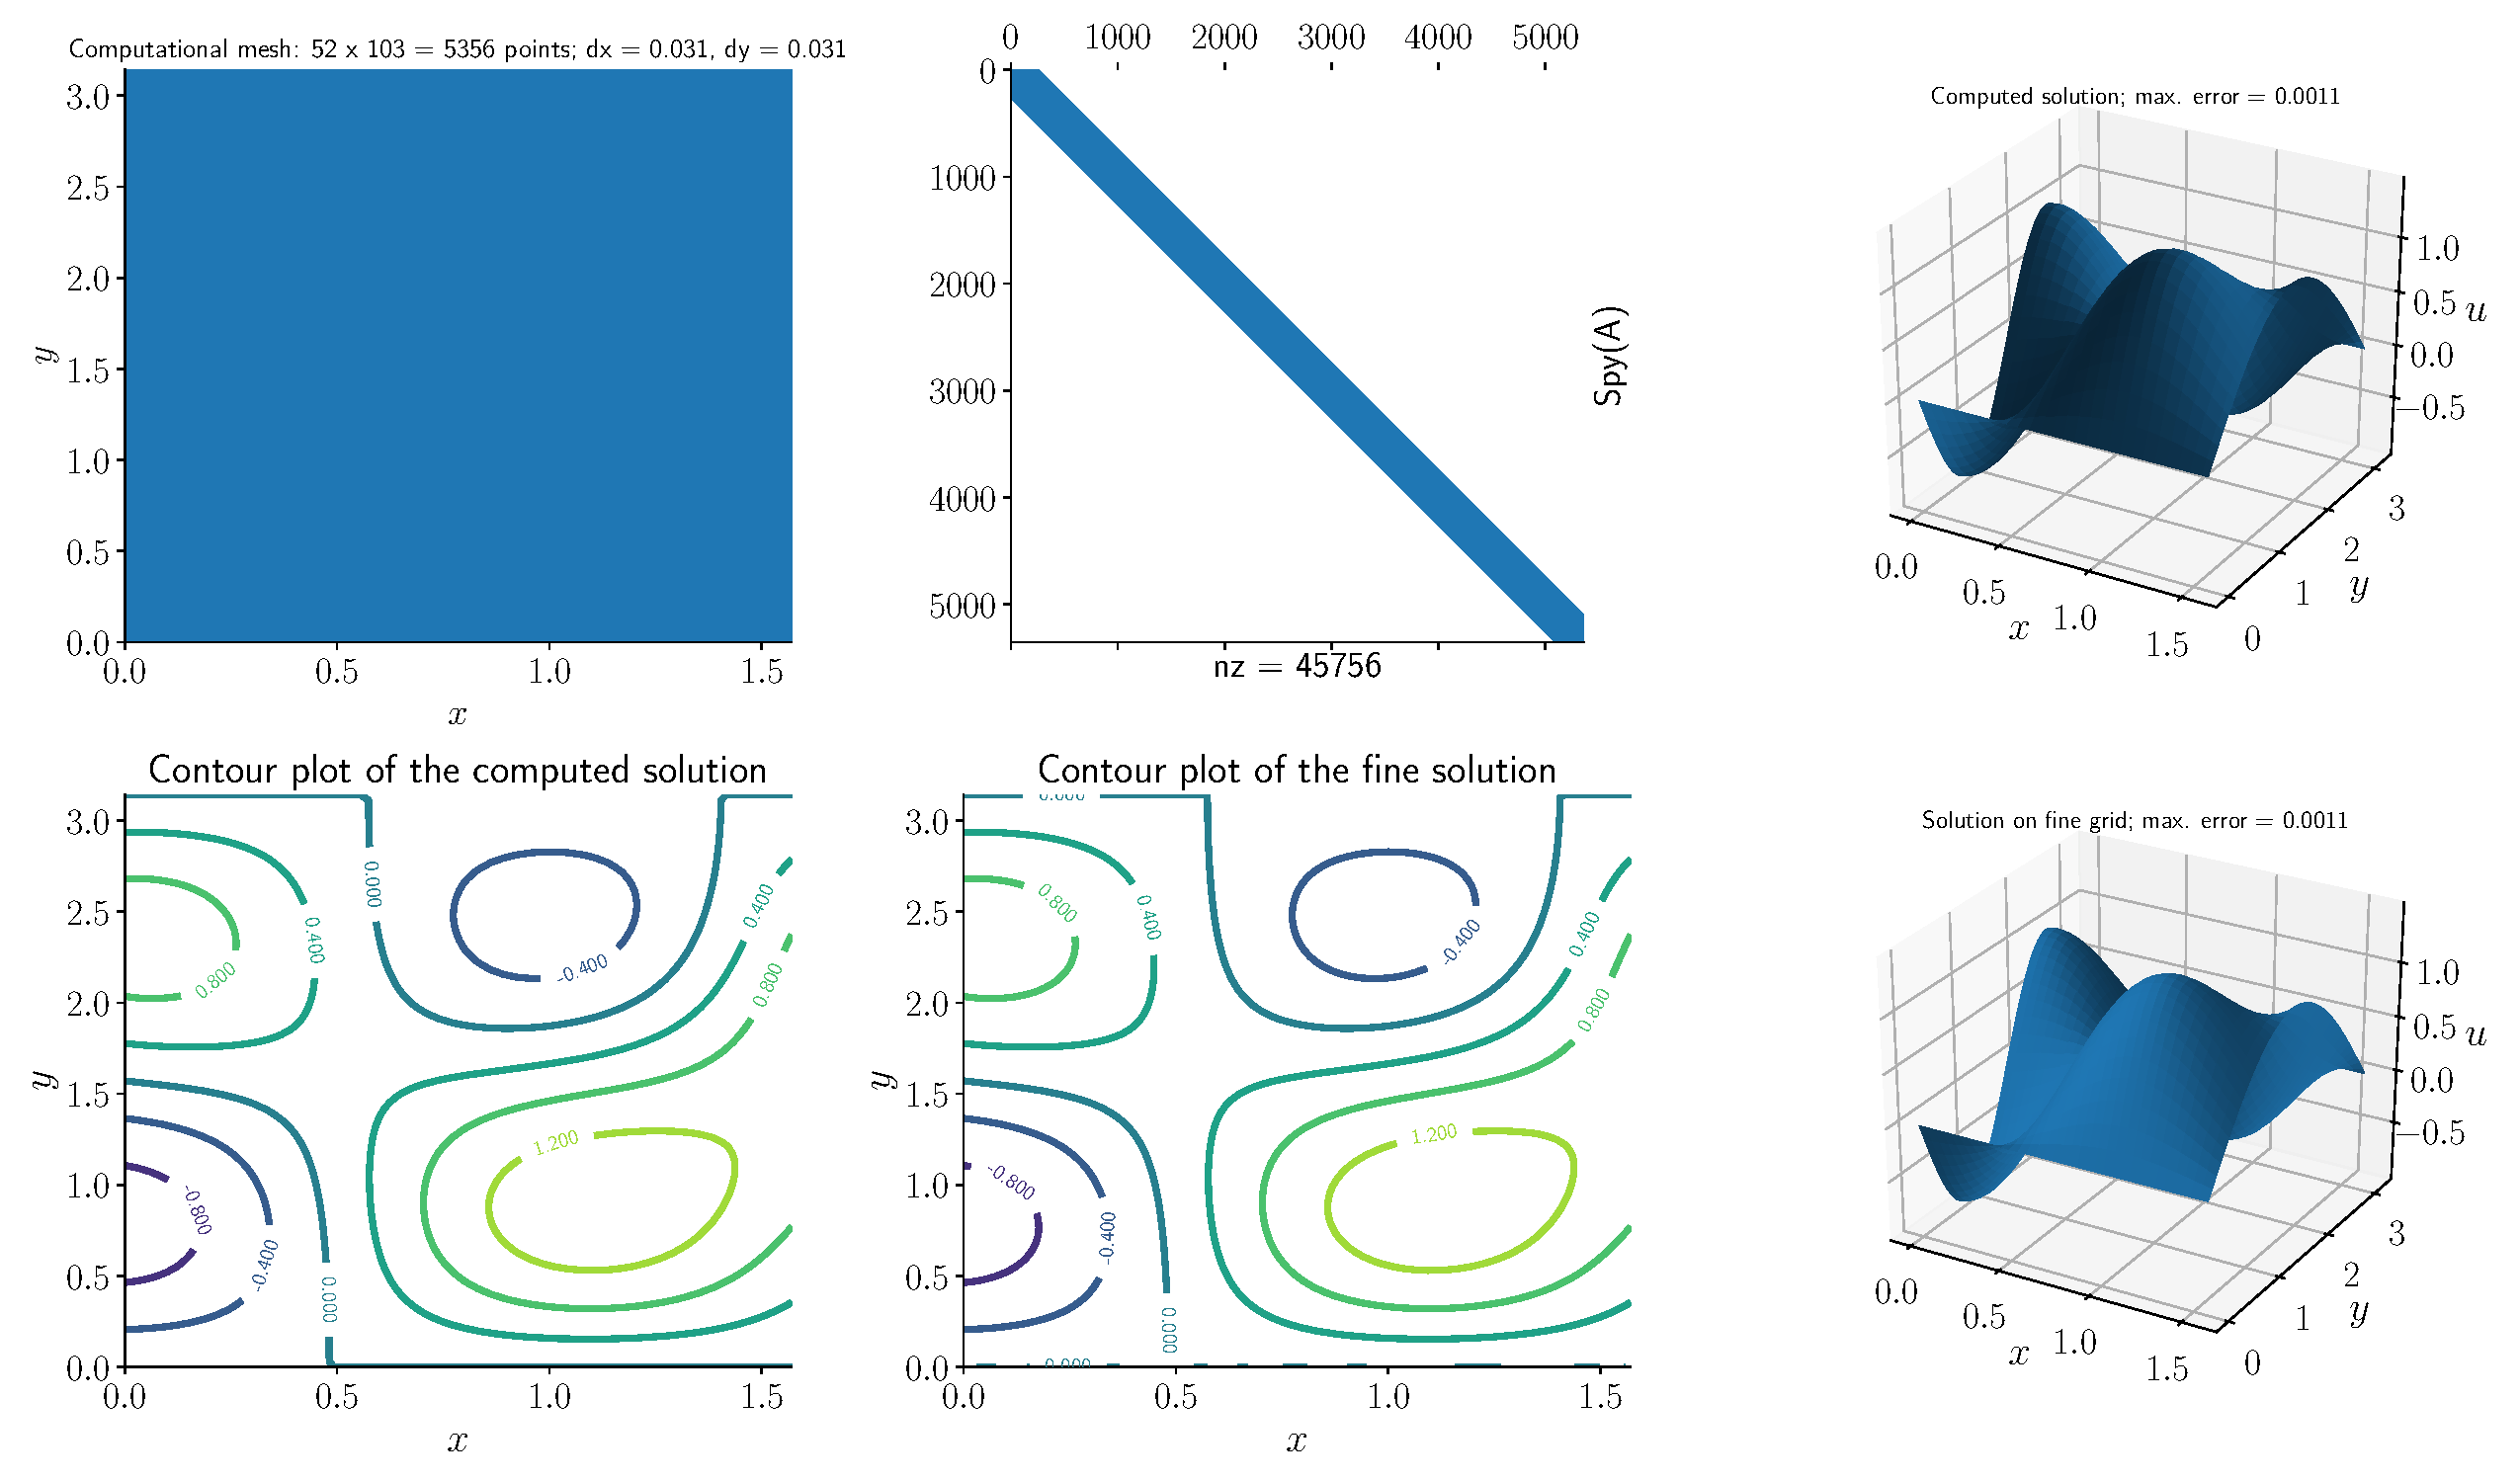
\includegraphics[clip,scale=0.4]{q2b_figure.pdf}
	\caption{Recreation of the example plots using the 9-point Laplacian.}
	\label{fig:nine_pt_soln_subplots}
\end{figure}

Like the 5-point Laplacian, this implementation of the 9-point Laplacian yields an observed accuracy order of two, which can be seen in Fig.~\ref{fig:nine_pt_err_scaling}.

\begin{figure}[!h]
	\centering
	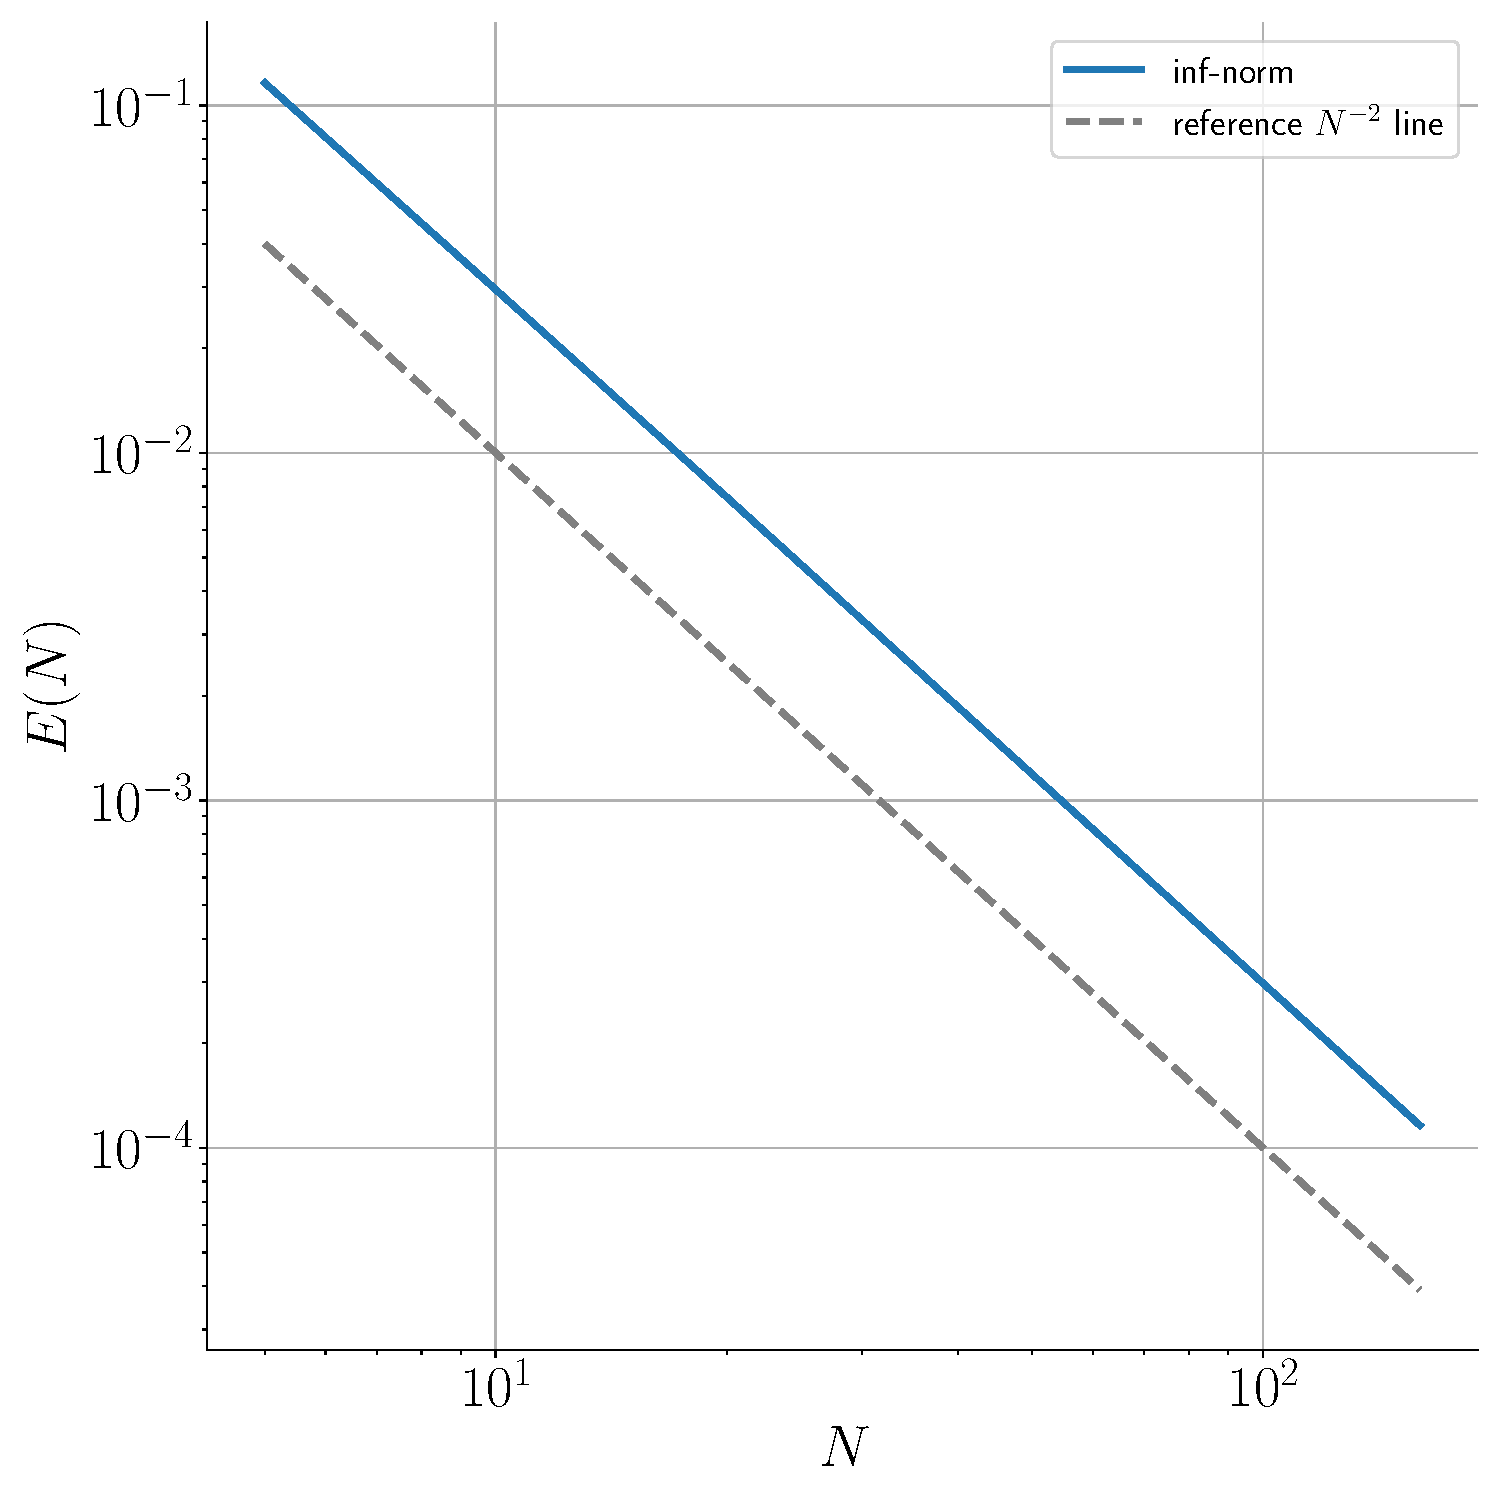
\includegraphics[clip,scale=0.4]{q2b_err_fig.pdf}
	\caption{Error, $E(N)$, as a function of the number of mesh intervals, $N$, for the nine-point Laplacian. We observe an order of two for the accuracy for this method.}
	\label{fig:nine_pt_err_scaling}
\end{figure}

\FloatBarrier

Implementing the deferred corrections by changing the right hand side of the PDE from,
\begin{subequations}
	\begin{align}
		f(x_{i},y_{j})&\to \tilde{f}(x_{i},y_{j})\\
		&= f(x_{i},y_{j}) + \dfrac{h^{2}}{12}\laplacian{f(x_{i},y_{j})}\\
		&= 13\cos(3x)\sin(2y) - \dfrac{h^{2}}{12}169\cos(3x)\sin(2y),
	\end{align}
\end{subequations}
we acquire the error scaling observed in Fig.~\ref{fig:nine_pt_deferred_err_scaling}. We observe that this correction increases the order of the method by two from two to four. From the grid refinement (see ipython notebook), I estimate that we would need 350 grid points in the $x$-direction and correspondingly $700$ grid points in the y-direction to acquire an inf-norm error of $< 10^{-5}$.

\begin{figure}[!h]
	\centering
	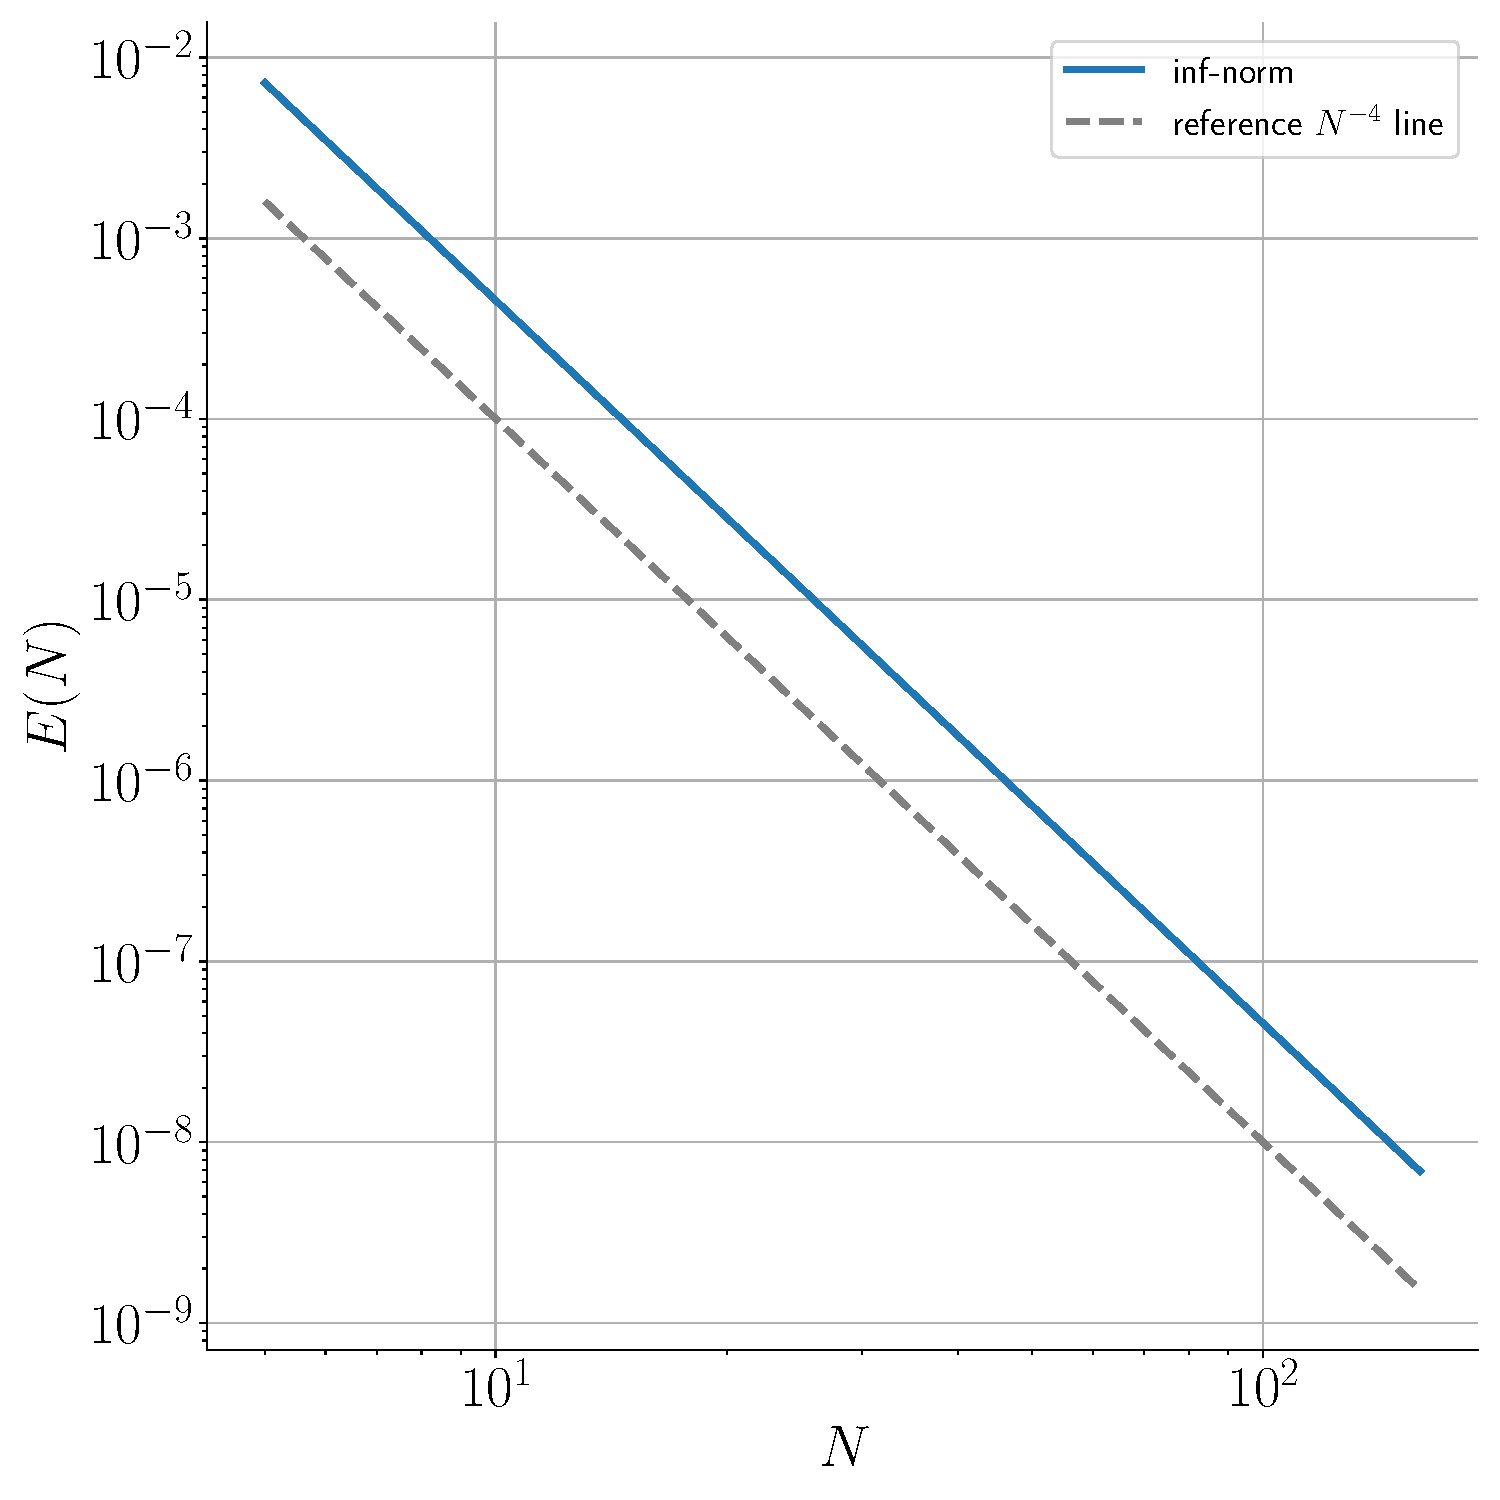
\includegraphics[clip,scale=0.4]{q2b_deferred_err_fig.pdf}
	\caption{Error, $E(N)$, as a function of the number of mesh intervals, $N$, for the nine-point Laplacian with deferred corrections. We observe the desired order of four for this method.}
	\label{fig:nine_pt_deferred_err_scaling}
\end{figure}

\subsection*{Part C}

We implement the Neumann Boundary condition using a second-order one-sided difference approximation so that
\begin{align}
	u_{x}(x=0,y_{j}) &\approx \dfrac{1}{h}\left[-\dfrac{3}{2}U_{0,j}+2U_{1,j}-\dfrac{1}{2}U_{2,j}\right] = \dfrac{1}{2}\sin y_{j}.
\end{align}
Performing grid refinement on the implementation of the Neumann boundary condition using the five-point stencil, gives the desired order of two as can be seen in Fig.~\ref{fig:neumann_err_scaling}. I suspect that the reason why this method deviates from the order 2 scaling at low $N$ is because in those cases, the stencil of this boundary condition takes up the majority of points on the grid. 

\begin{figure}[!h]
	\centering
	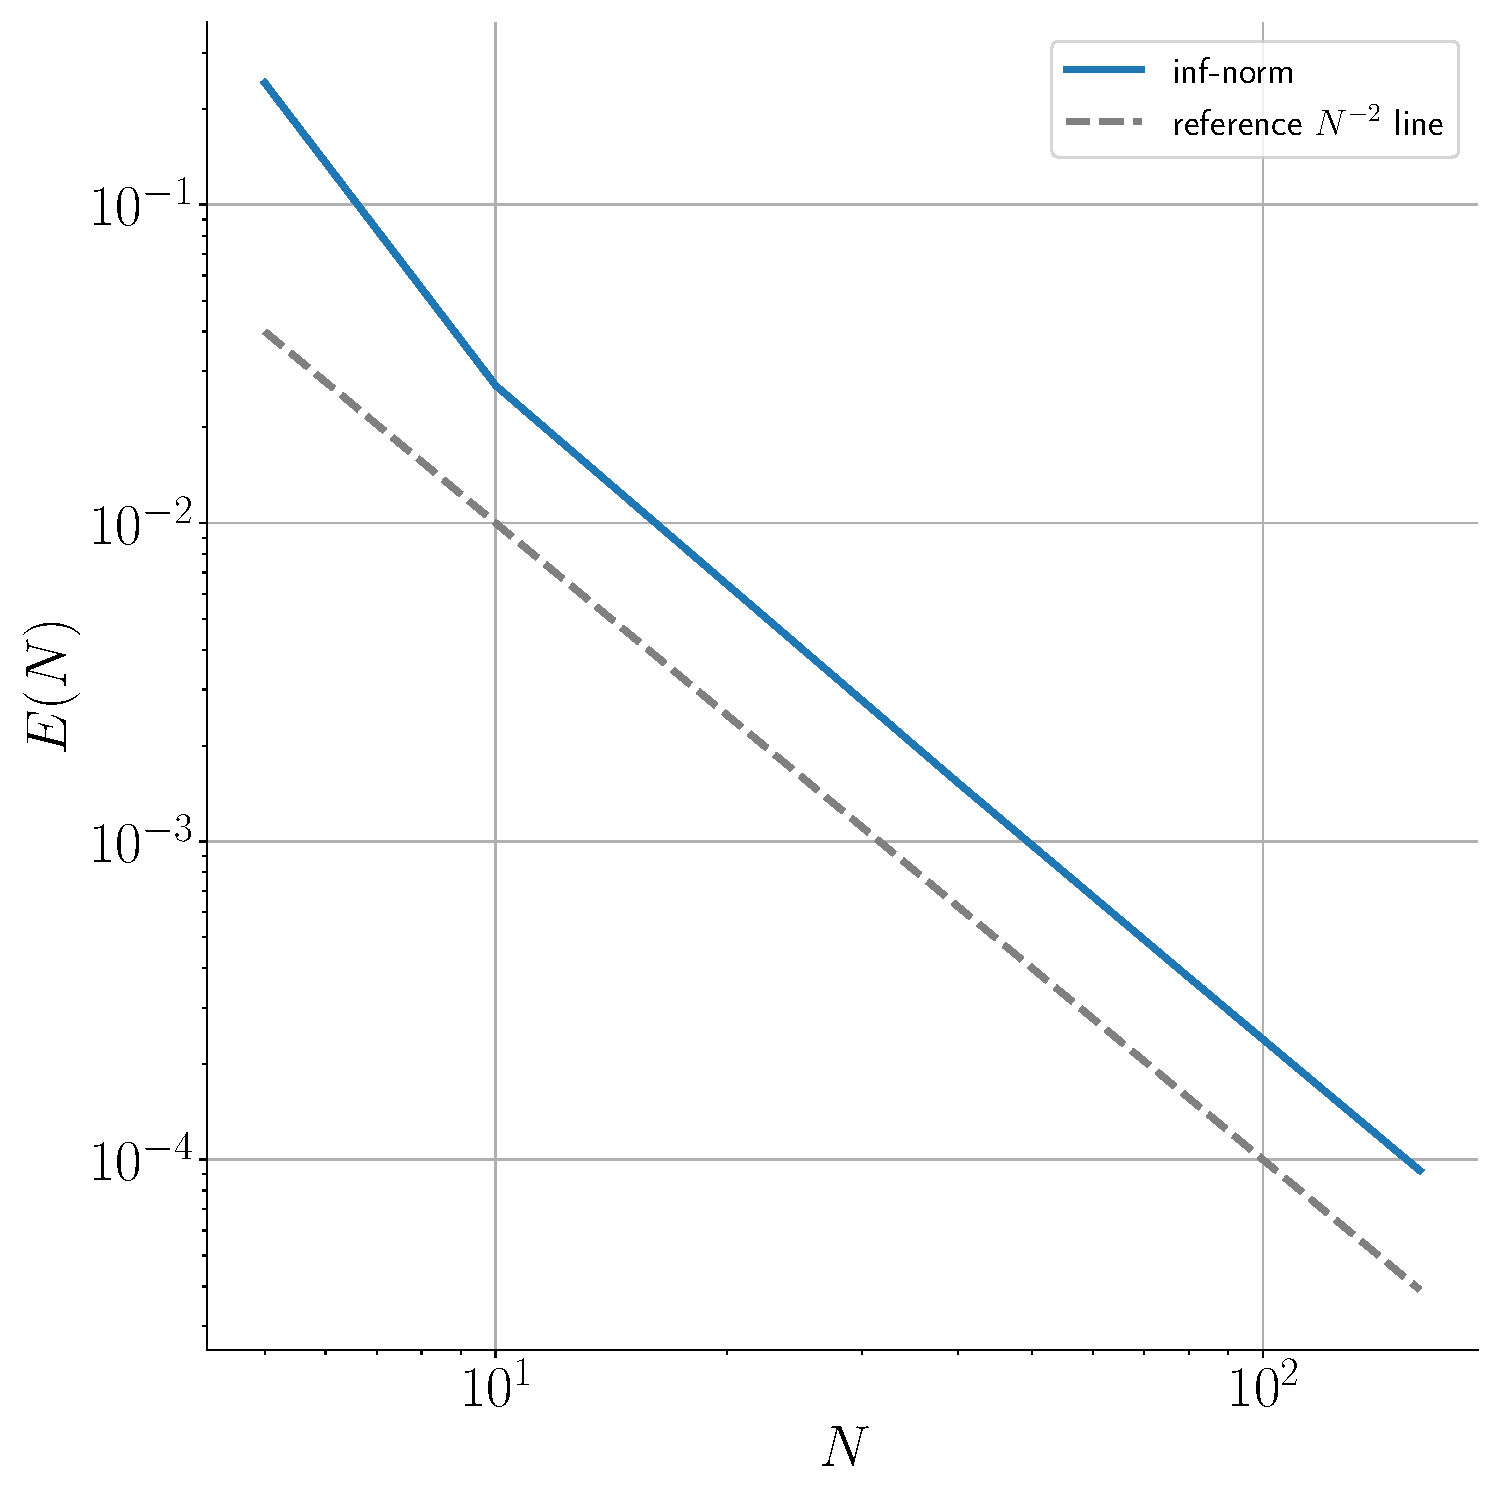
\includegraphics[clip,scale=0.4]{q2c_err_fig.pdf}
	\caption{Error, $E(N)$, as a function of the number of mesh intervals, $N$, for the five-point Laplacian with Neumann boundary conditions at $x=0$. We observe the desired order of two for this method.}
	\label{fig:neumann_err_scaling}
\end{figure}

\end{document}